\documentclass{beamer}
\usetheme{metropolis}           % Use metropolis theme

\title{Brain Age Prediction Models}
\date{\today}
\author{Diego Rodrigues}

\begin{document}

% Title Page
\maketitle

% Table of Contents
\begin{frame}{Outline}
  \tableofcontents
\end{frame}

\begin{frame}{Common Prediction Models}
  \begin{itemize}
    \item \textbf{Machine Learning Approaches:}
      \begin{itemize}
        \item Support Vector Machines (SVM)
        \item Random Forests
        \item Neural Networks
      \end{itemize}
    \item \textbf{Deep Learning Approaches:}
      \begin{itemize}
        \item Convolutional Neural Networks (CNN)
        \item Recurrent Neural Networks (RNN)
      \end{itemize}
    \item \textbf{Feature Selection}
      \begin{itemize}
        \item MRI-derived features
        \item Cognitive and behavioral data
      \end{itemize}
  \end{itemize}
\end{frame}

\begin{frame}{Challenges in Brain Age Prediction}
  \begin{itemize}
    \item \textbf{Data Heterogeneity:} Variability in datasets and imaging protocols.
    \item \textbf{Model Generalizability:} Overfitting and applicability to different populations.
    \item \textbf{Interpretability:} Understanding what drives the predictions.
  \end{itemize}
\end{frame}

% Section: The Dallas Lifespan Brain Study
\section{The Dallas Lifespan Brain Study}
\begin{frame}{Overview of the DLBS\cite{ds004856:1.0.0}}
  \begin{itemize}
    \item \textbf{Longitudinal multi-modal neuroimaging study initiated in 2008.}
    \item \textbf{Participants:} Ages 20-90, returning for three waves over approximately 10 years.
    \item \textbf{Data Collected:}
      \begin{itemize}
        \item Structural MRI, diffusion MRI, functional MRI.
        \item Amyloid and tau PET imaging.
        \item Comprehensive cognitive and psychosocial assessments.
      \end{itemize}
    \item \textbf{Aim:} Investigate MRI metrics related to brain aging and Alzheimer's disease biomarkers across the adult lifespan.
  \end{itemize}
\end{frame}

\begin{frame}{DLBS Data Acquisition}
  \begin{itemize}
    \item \textbf{Cognitive Measures:}
      \begin{itemize}
        \item Speed of Processing, Working Memory, Episodic Memory, Reasoning, Vocabulary, Verbal Fluency.
      \end{itemize}
    \item \textbf{Surveys:}
      \begin{itemize}
        \item Physical Health, Mental Health, Psychosocial Factors.
      \end{itemize}
    \item \textbf{MRI Protocol:}
      \begin{itemize}
        \item Functional tasks (Ventral Visual Task, Words Task, Scenes Task).
        \item Structural imaging (MPRAGE, FLAIR).
        \item Resting-state imaging, Diffusion Tensor Imaging (DTI), Arterial Spin Labeling (ASL).
      \end{itemize}
    \item \textbf{PET Imaging:}
      \begin{itemize}
        \item Amyloid PET using 18F-AV-45 (florbetapir).
        \item Tau PET using 18F-AV-1451 (flortaucipir).
      \end{itemize}
  \end{itemize}
\end{frame}


% Section: Data Analysis using DLBS
\section{Data Analysis using DLBS}
\subsection{Demographics}
\begin{frame}{Participant Demographics}
  \begin{itemize}
    \item \textbf{Age Range:} 20-90 years old.
    \item \textbf{Participants:} around 500 individuals at Wave 1 and 200 at Wave 3
    \item \textbf{Inclusion Criteria:} Right-handed, fluent in English, etc.
    \item \textbf{Exclusion Criteria:} MMSE score below threshold, major psychiatric or neurological disorders, etc.
  \end{itemize}
\end{frame}

% Slide: Age Distribution
\begin{frame}{Age Distribution at Wave 1 MRI}
  \begin{figure}
    \centering
    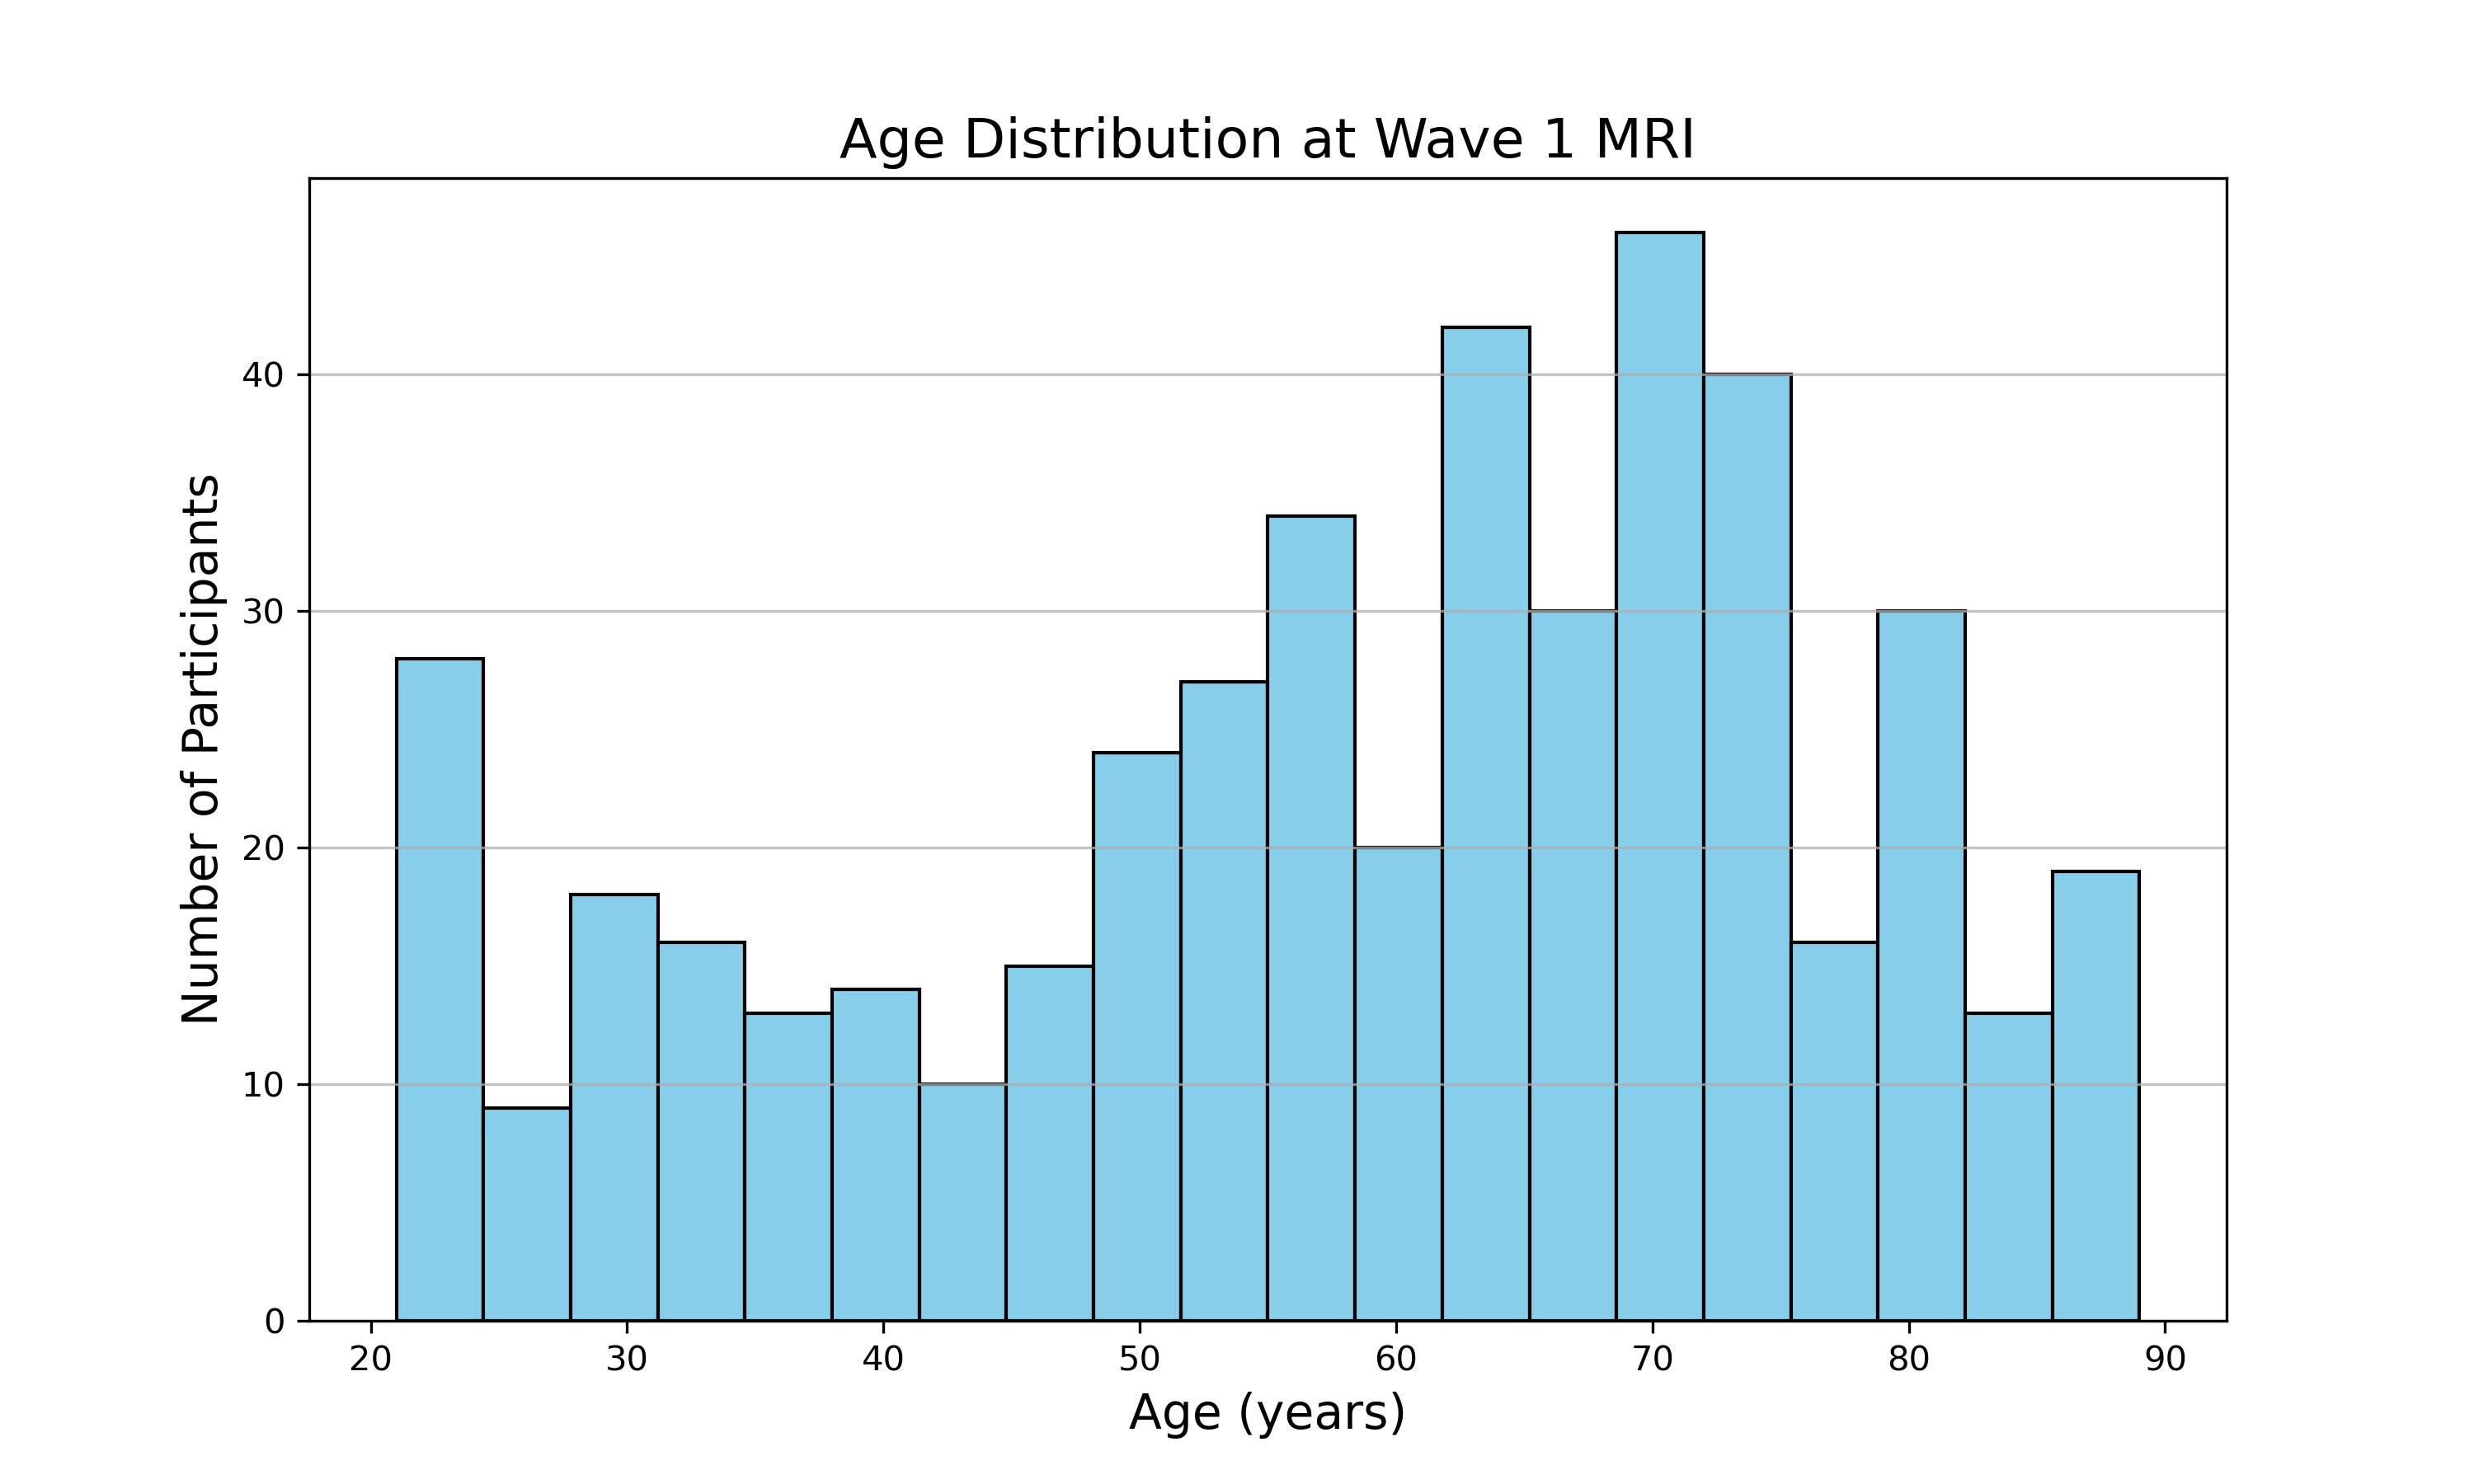
\includegraphics[width=0.8\linewidth]{age_distribution.png}
    \caption{Histogram of participants' age at Wave 1 MRI}
  \end{figure}
\end{frame}

% Slide: Sex Distribution
\begin{frame}{Sex Distribution of Participants}
  \begin{figure}
    \centering
    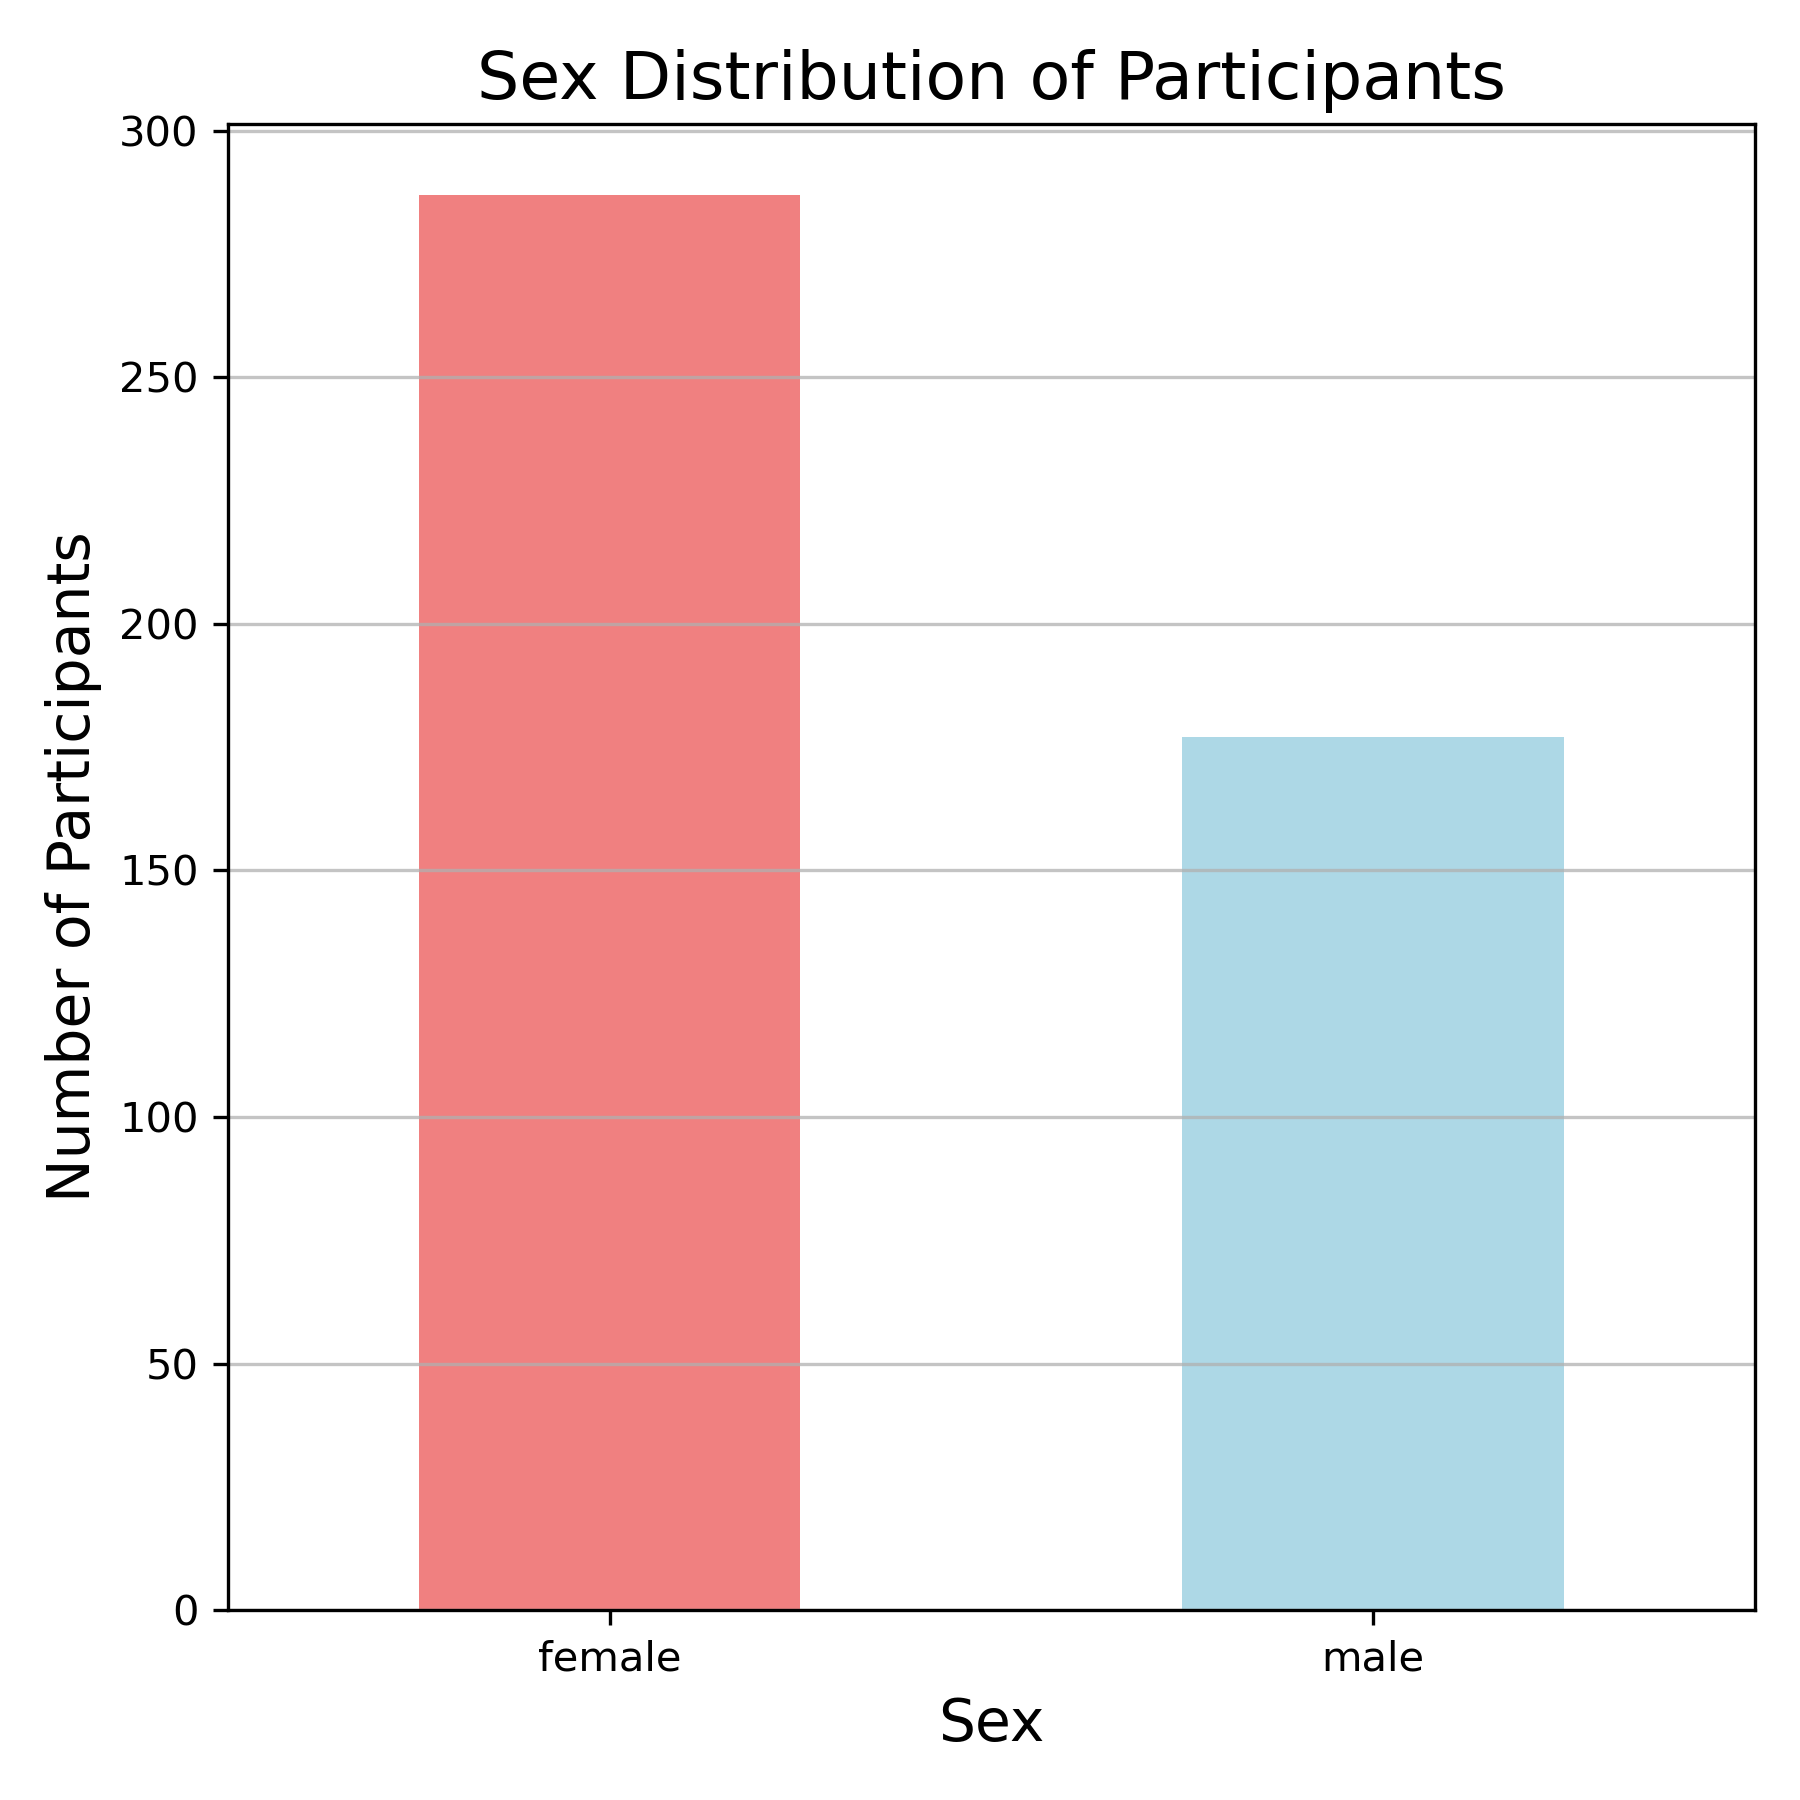
\includegraphics[width=0.6\linewidth]{sex_distribution.png}
    \caption{Bar chart of participants' sex distribution}
  \end{figure}
\end{frame}

% Slide: Race Distribution
\begin{frame}{Race Distribution of Participants}
  \begin{figure}
    \centering
    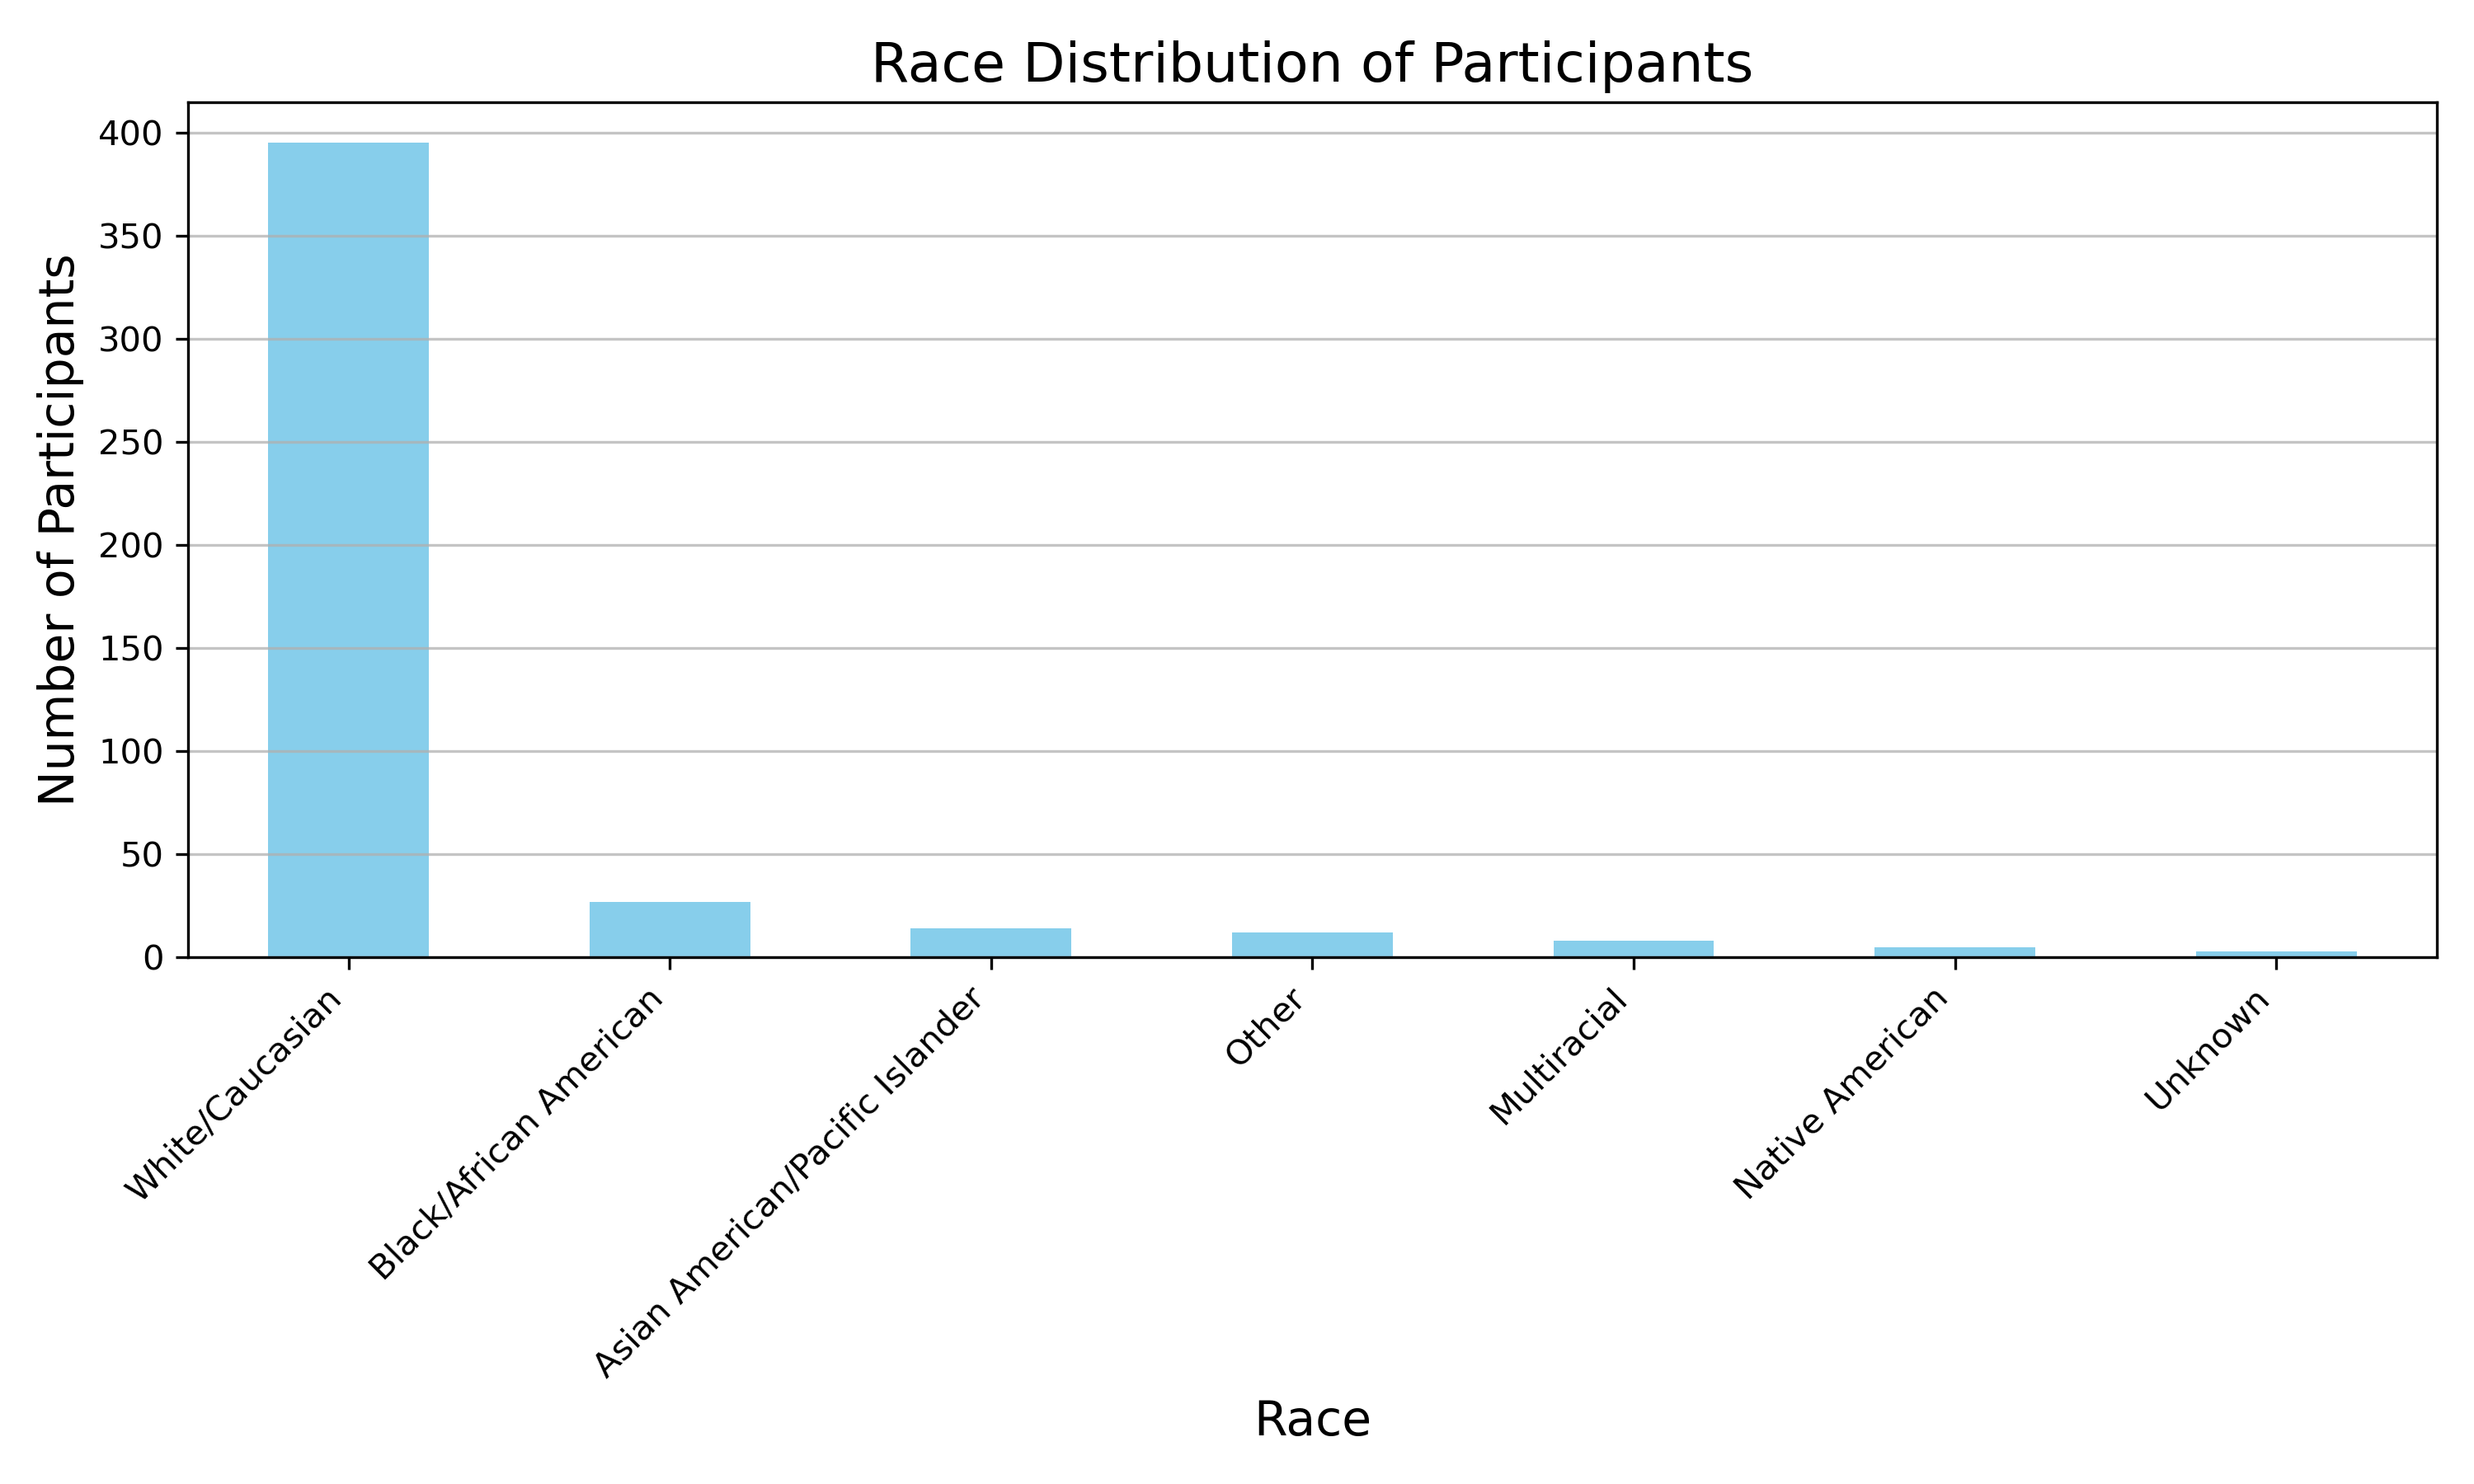
\includegraphics[width=0.8\linewidth]{race_distribution.png}
    \caption{Bar chart of participants' race distribution}
  \end{figure}
\end{frame}

% Subsection: Health Metrics
\subsection{Health Metrics}

% Slide: BMI Distribution
\begin{frame}{BMI Distribution at Wave 1}
  \begin{figure}
    \centering
    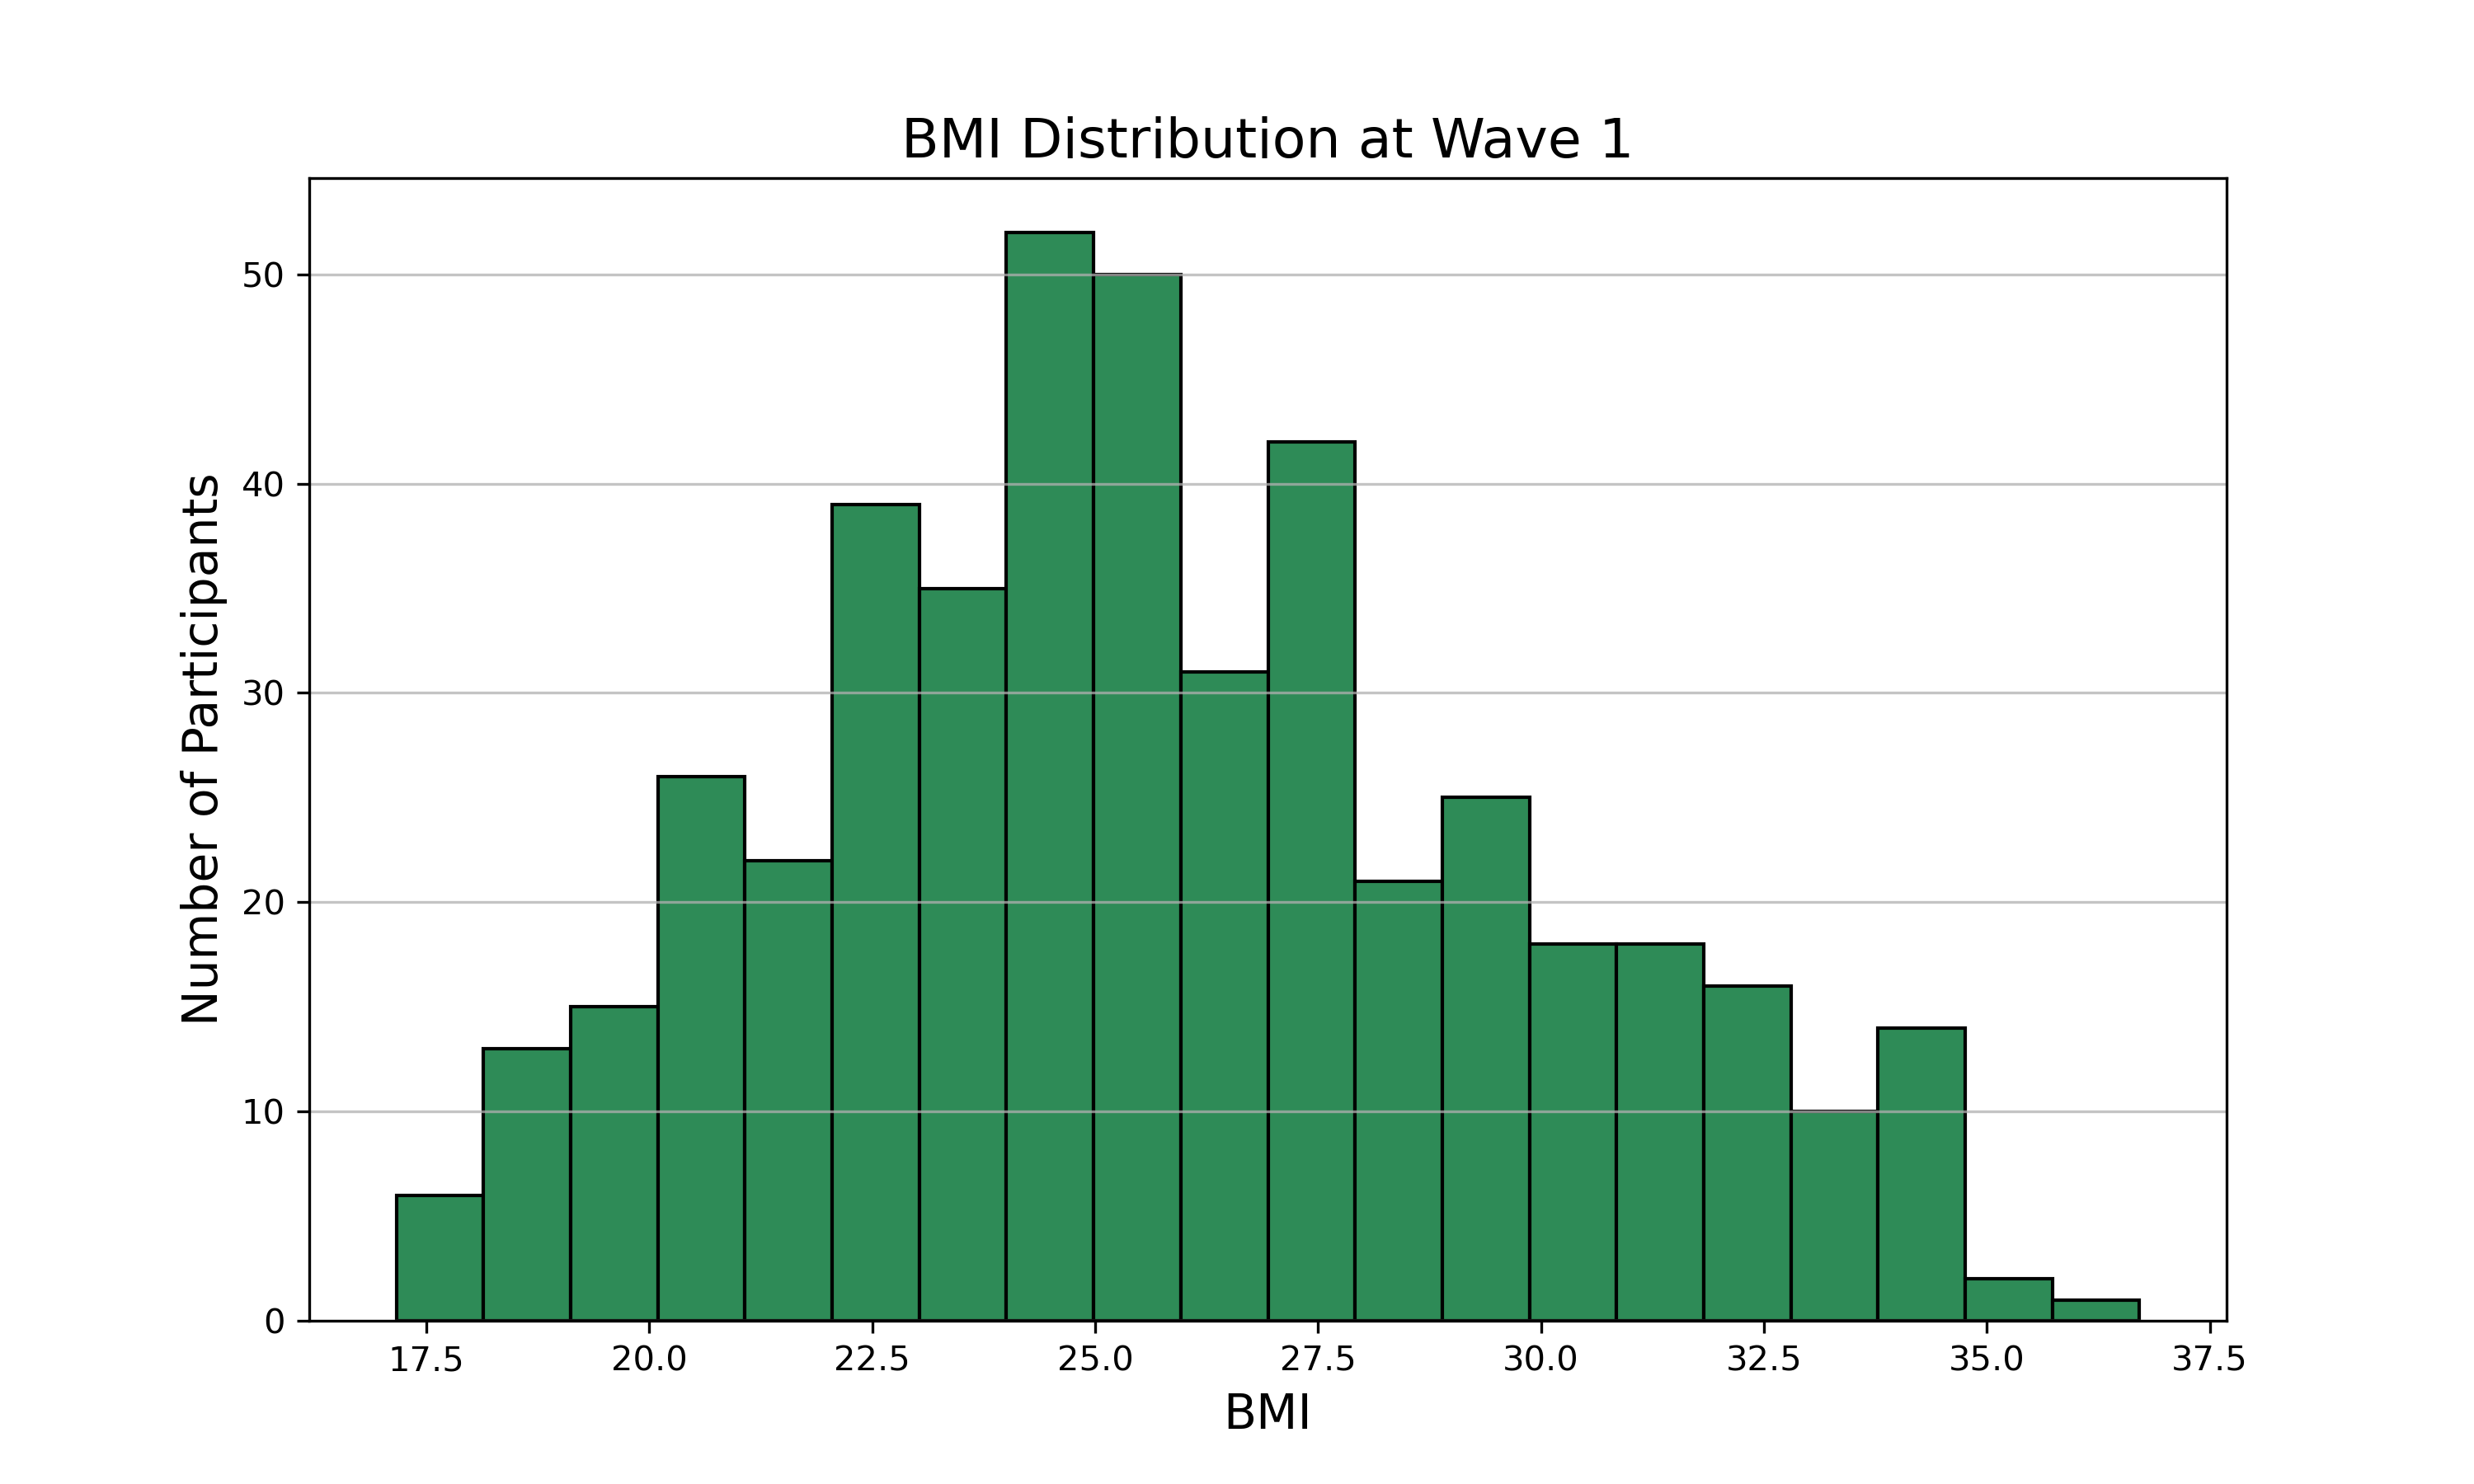
\includegraphics[width=0.8\linewidth]{bmi_distribution.png}
    \caption{Histogram of BMI at Wave 1}
  \end{figure}
\end{frame}

% Slide: Age vs. BMI Scatter Plot
\begin{frame}{Age vs. BMI at Wave 1}
  \begin{figure}
    \centering
    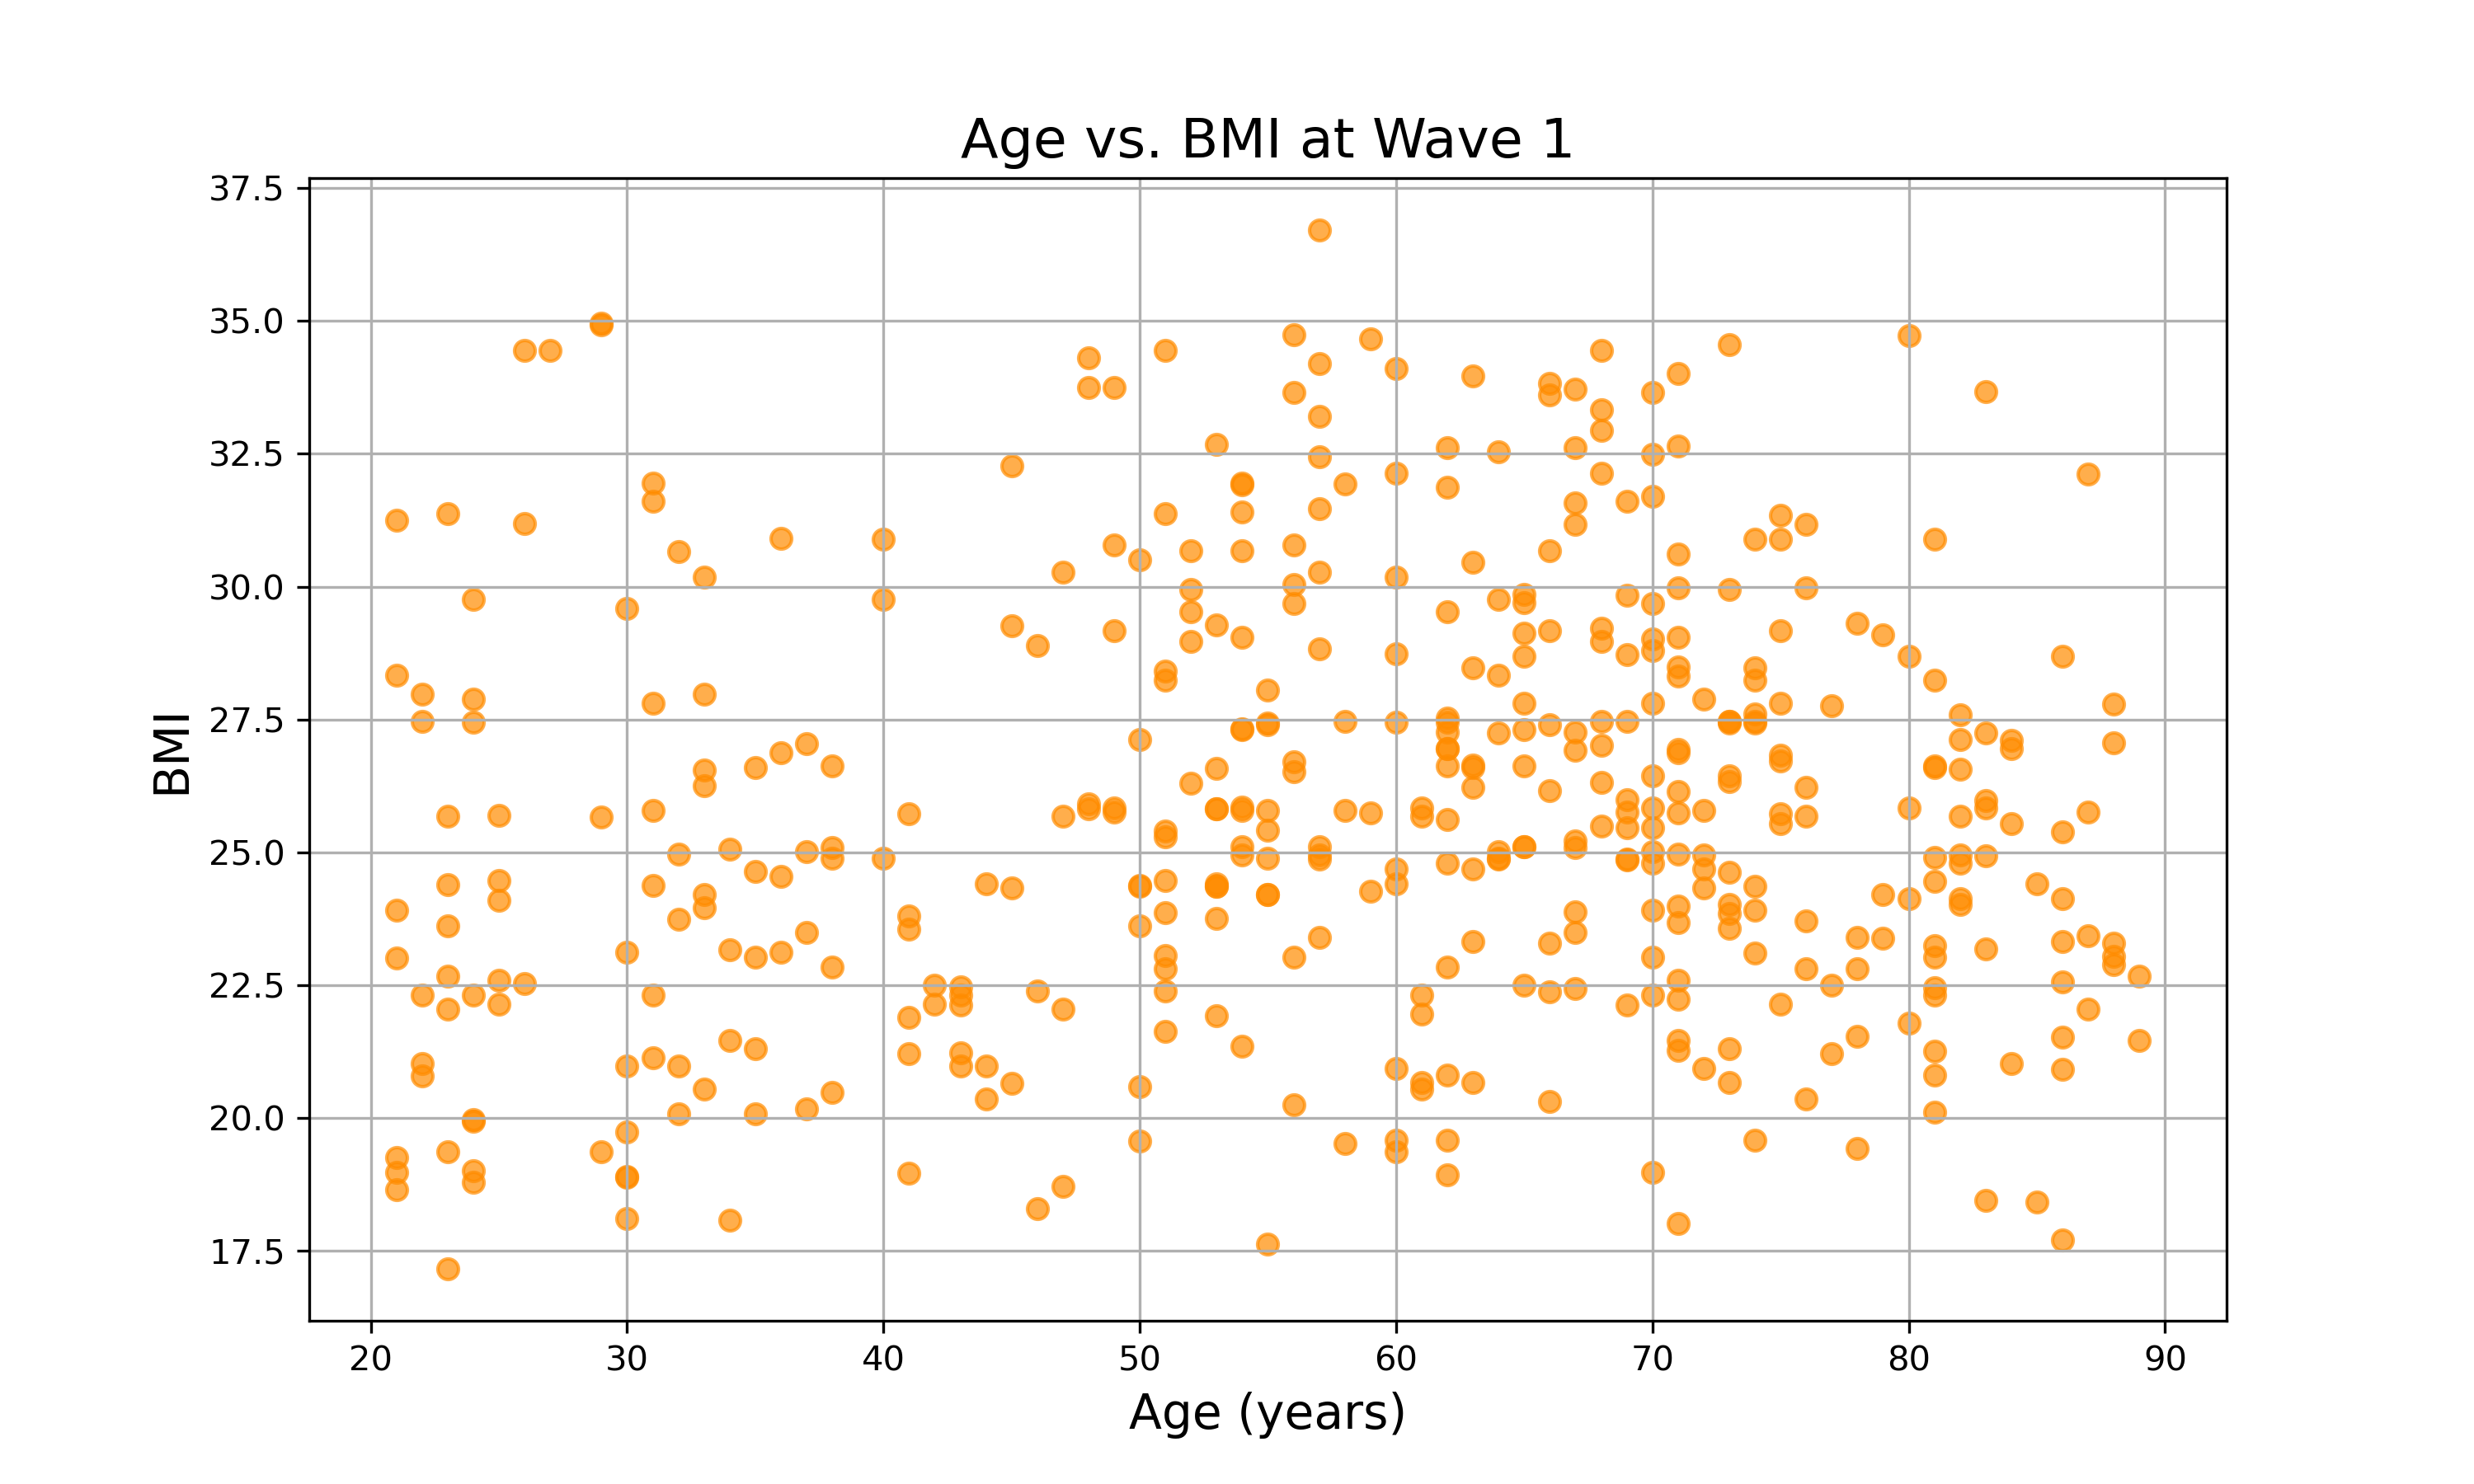
\includegraphics[width=0.8\linewidth]{age_vs_bmi_w1.png}
    \caption{Scatter plot of Age vs. BMI at Wave 1}
  \end{figure}
\end{frame}

% Subsection: Cognitive Function
\subsection{Cognitive Function}

% Slide: MMSE Score Distribution at Wave 1
\begin{frame}{MMSE Score Distribution at Wave 1}
  \begin{figure}
    \centering
    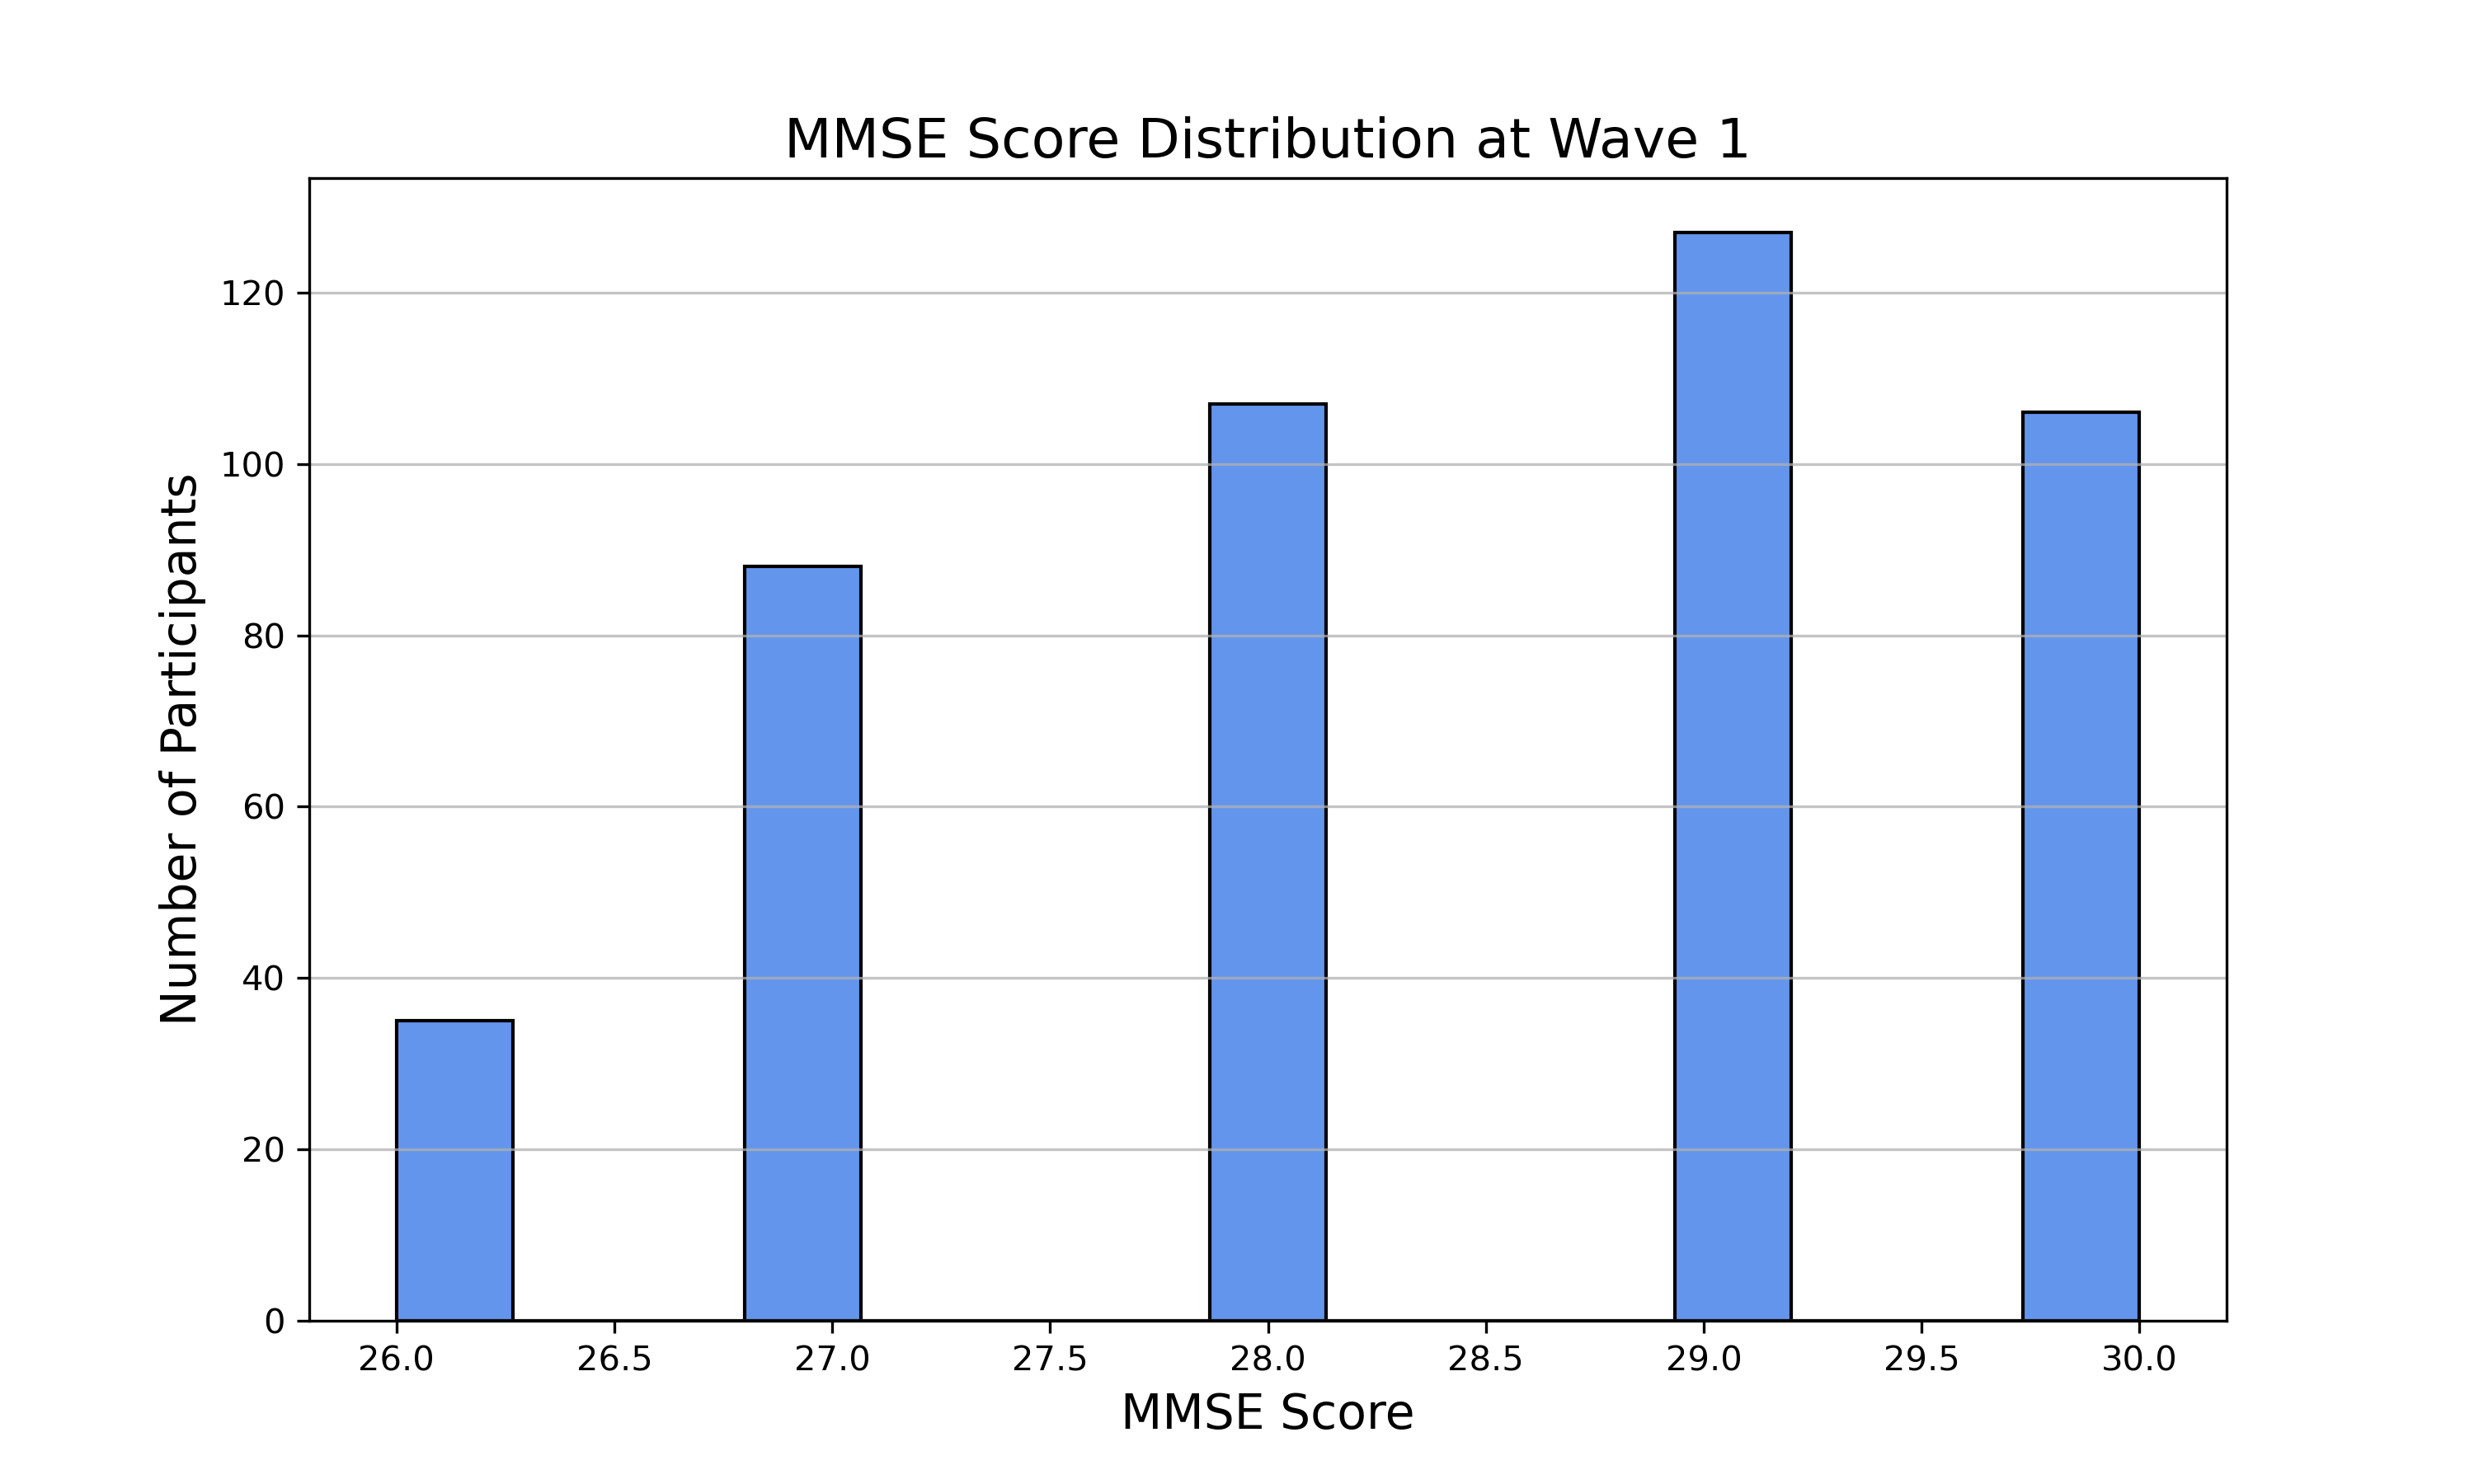
\includegraphics[width=0.8\linewidth]{mmse_w1_distribution.png}
    \caption{Histogram of MMSE scores at Wave 1}
  \end{figure}
\end{frame}

% Slide: MMSE Score Distribution at Wave 2
\begin{frame}{MMSE Score Distribution at Wave 2}
  \begin{figure}
    \centering
    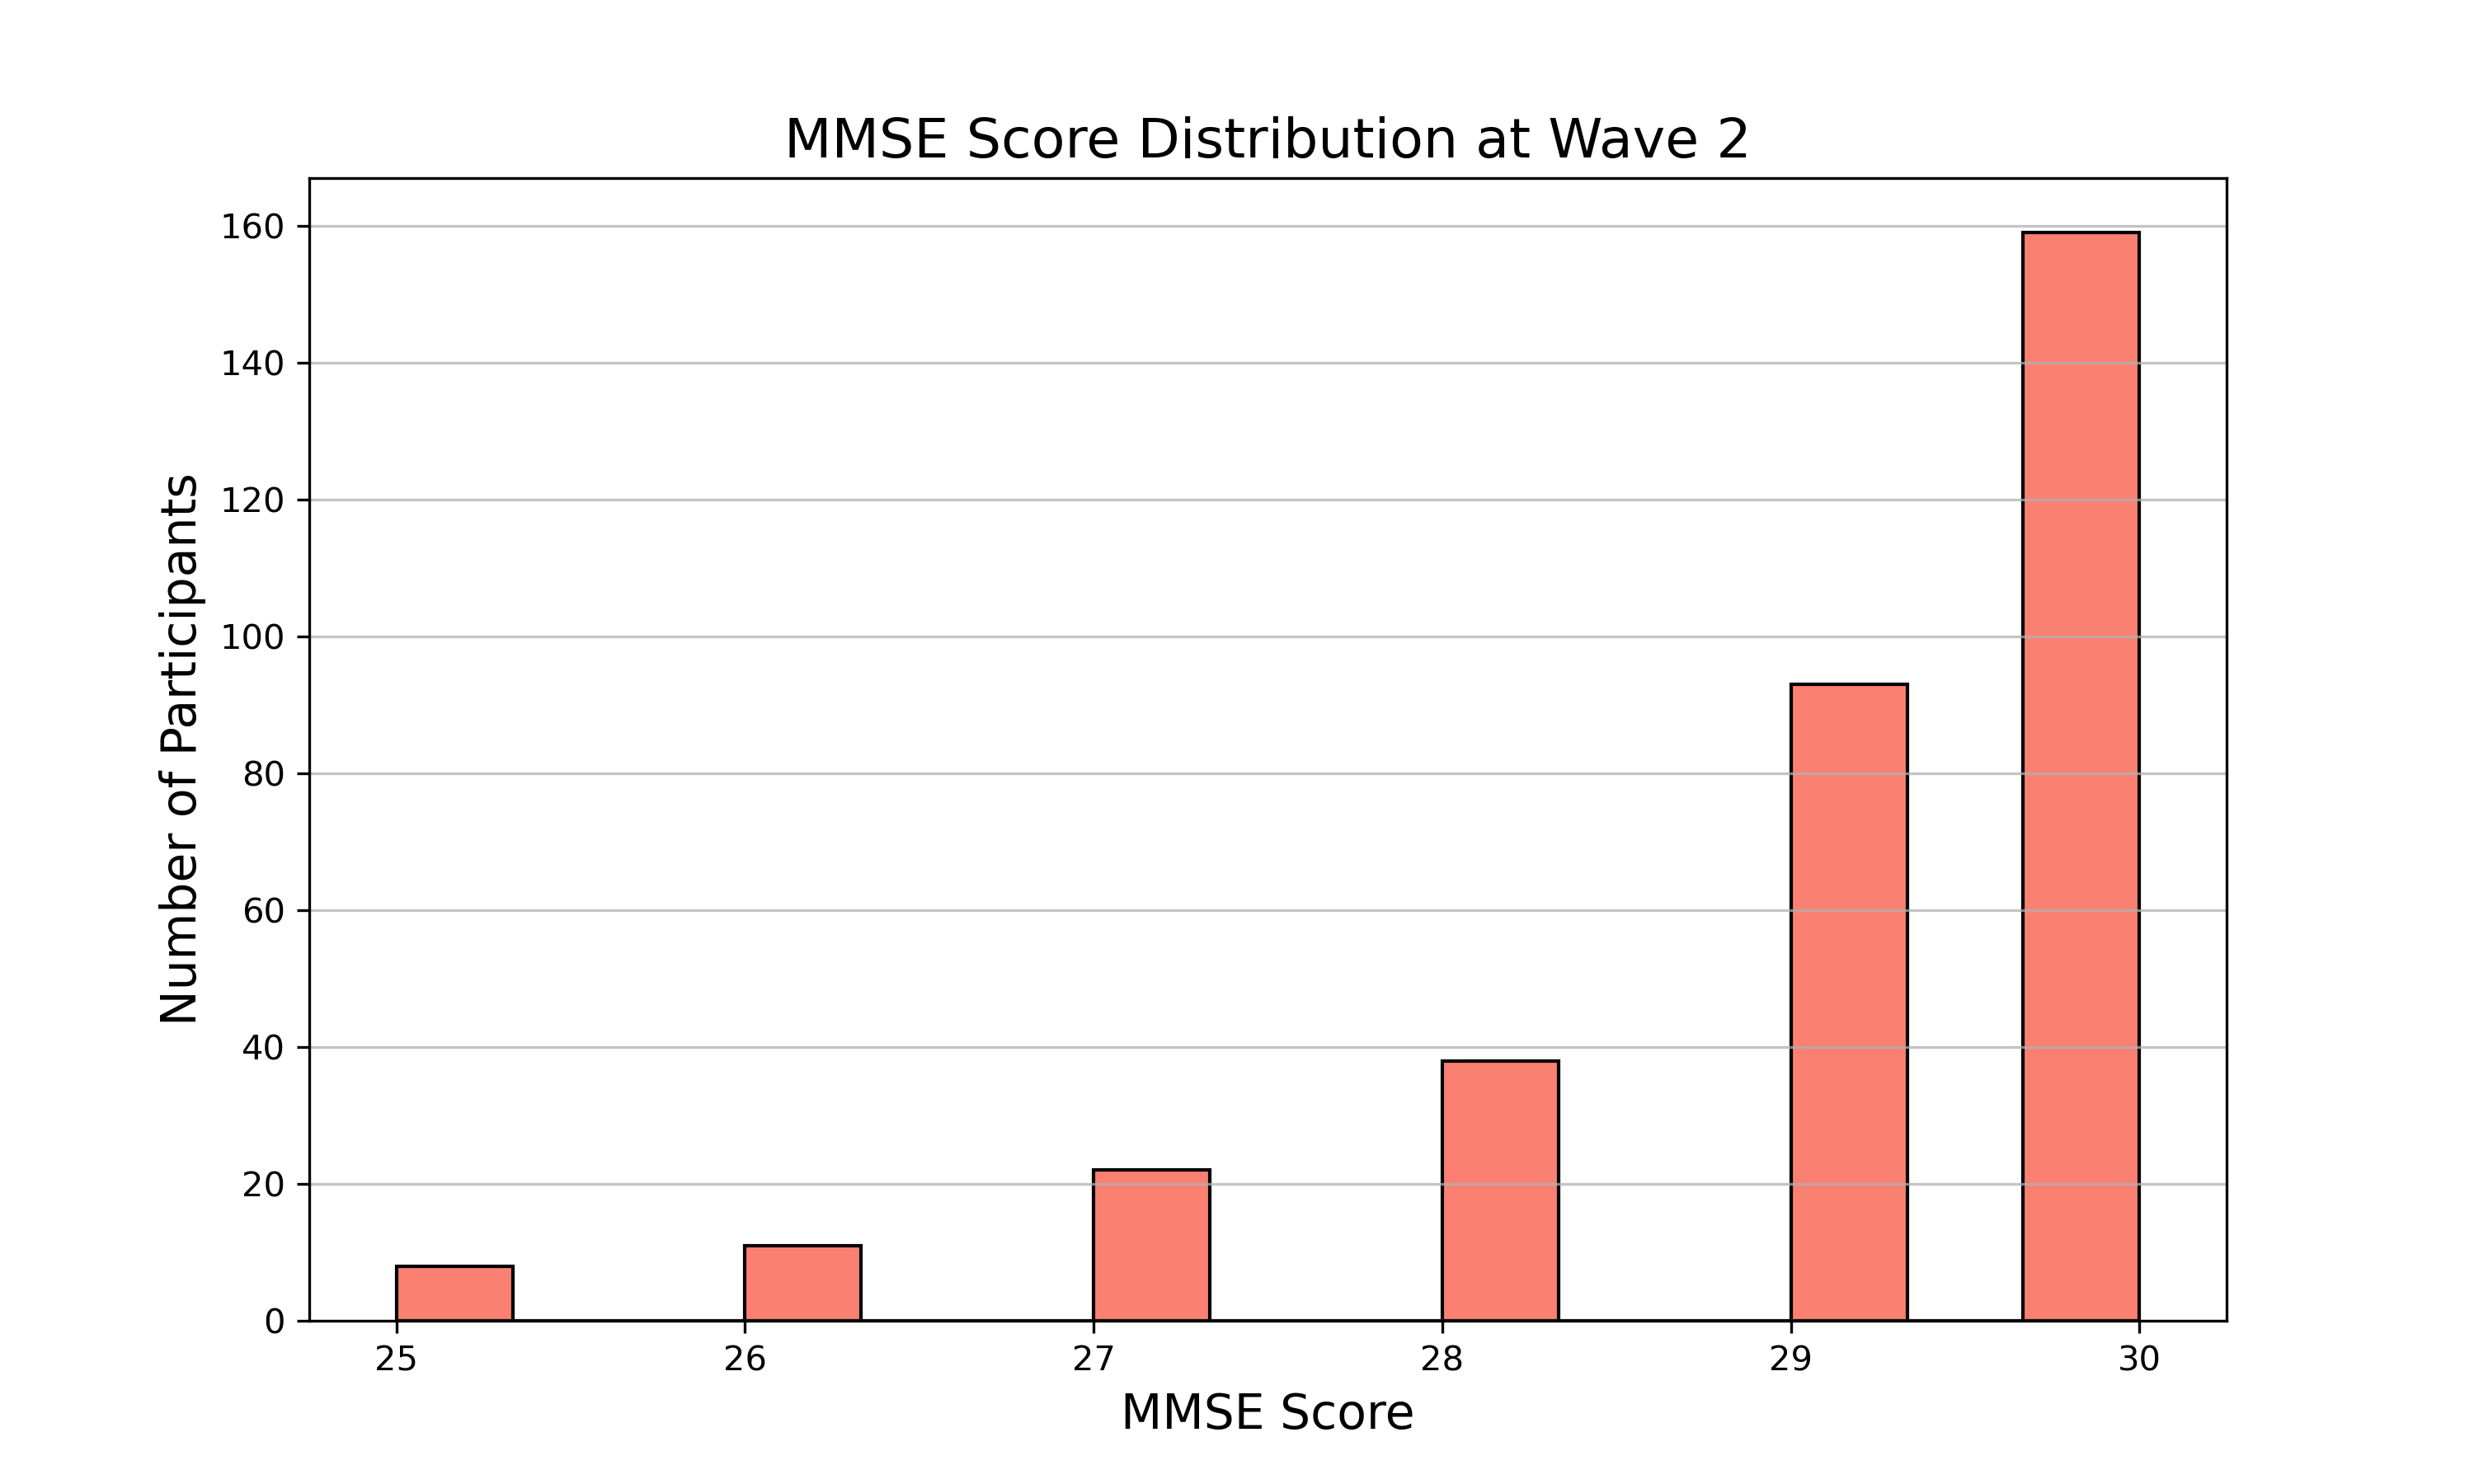
\includegraphics[width=0.8\linewidth]{mmse_w2_distribution.png}
    \caption{Histogram of MMSE scores at Wave 2}
  \end{figure}
\end{frame}

% Slide: MMSE Score Distribution at Wave 3
\begin{frame}{MMSE Score Distribution at Wave 3}
  \begin{figure}
    \centering
    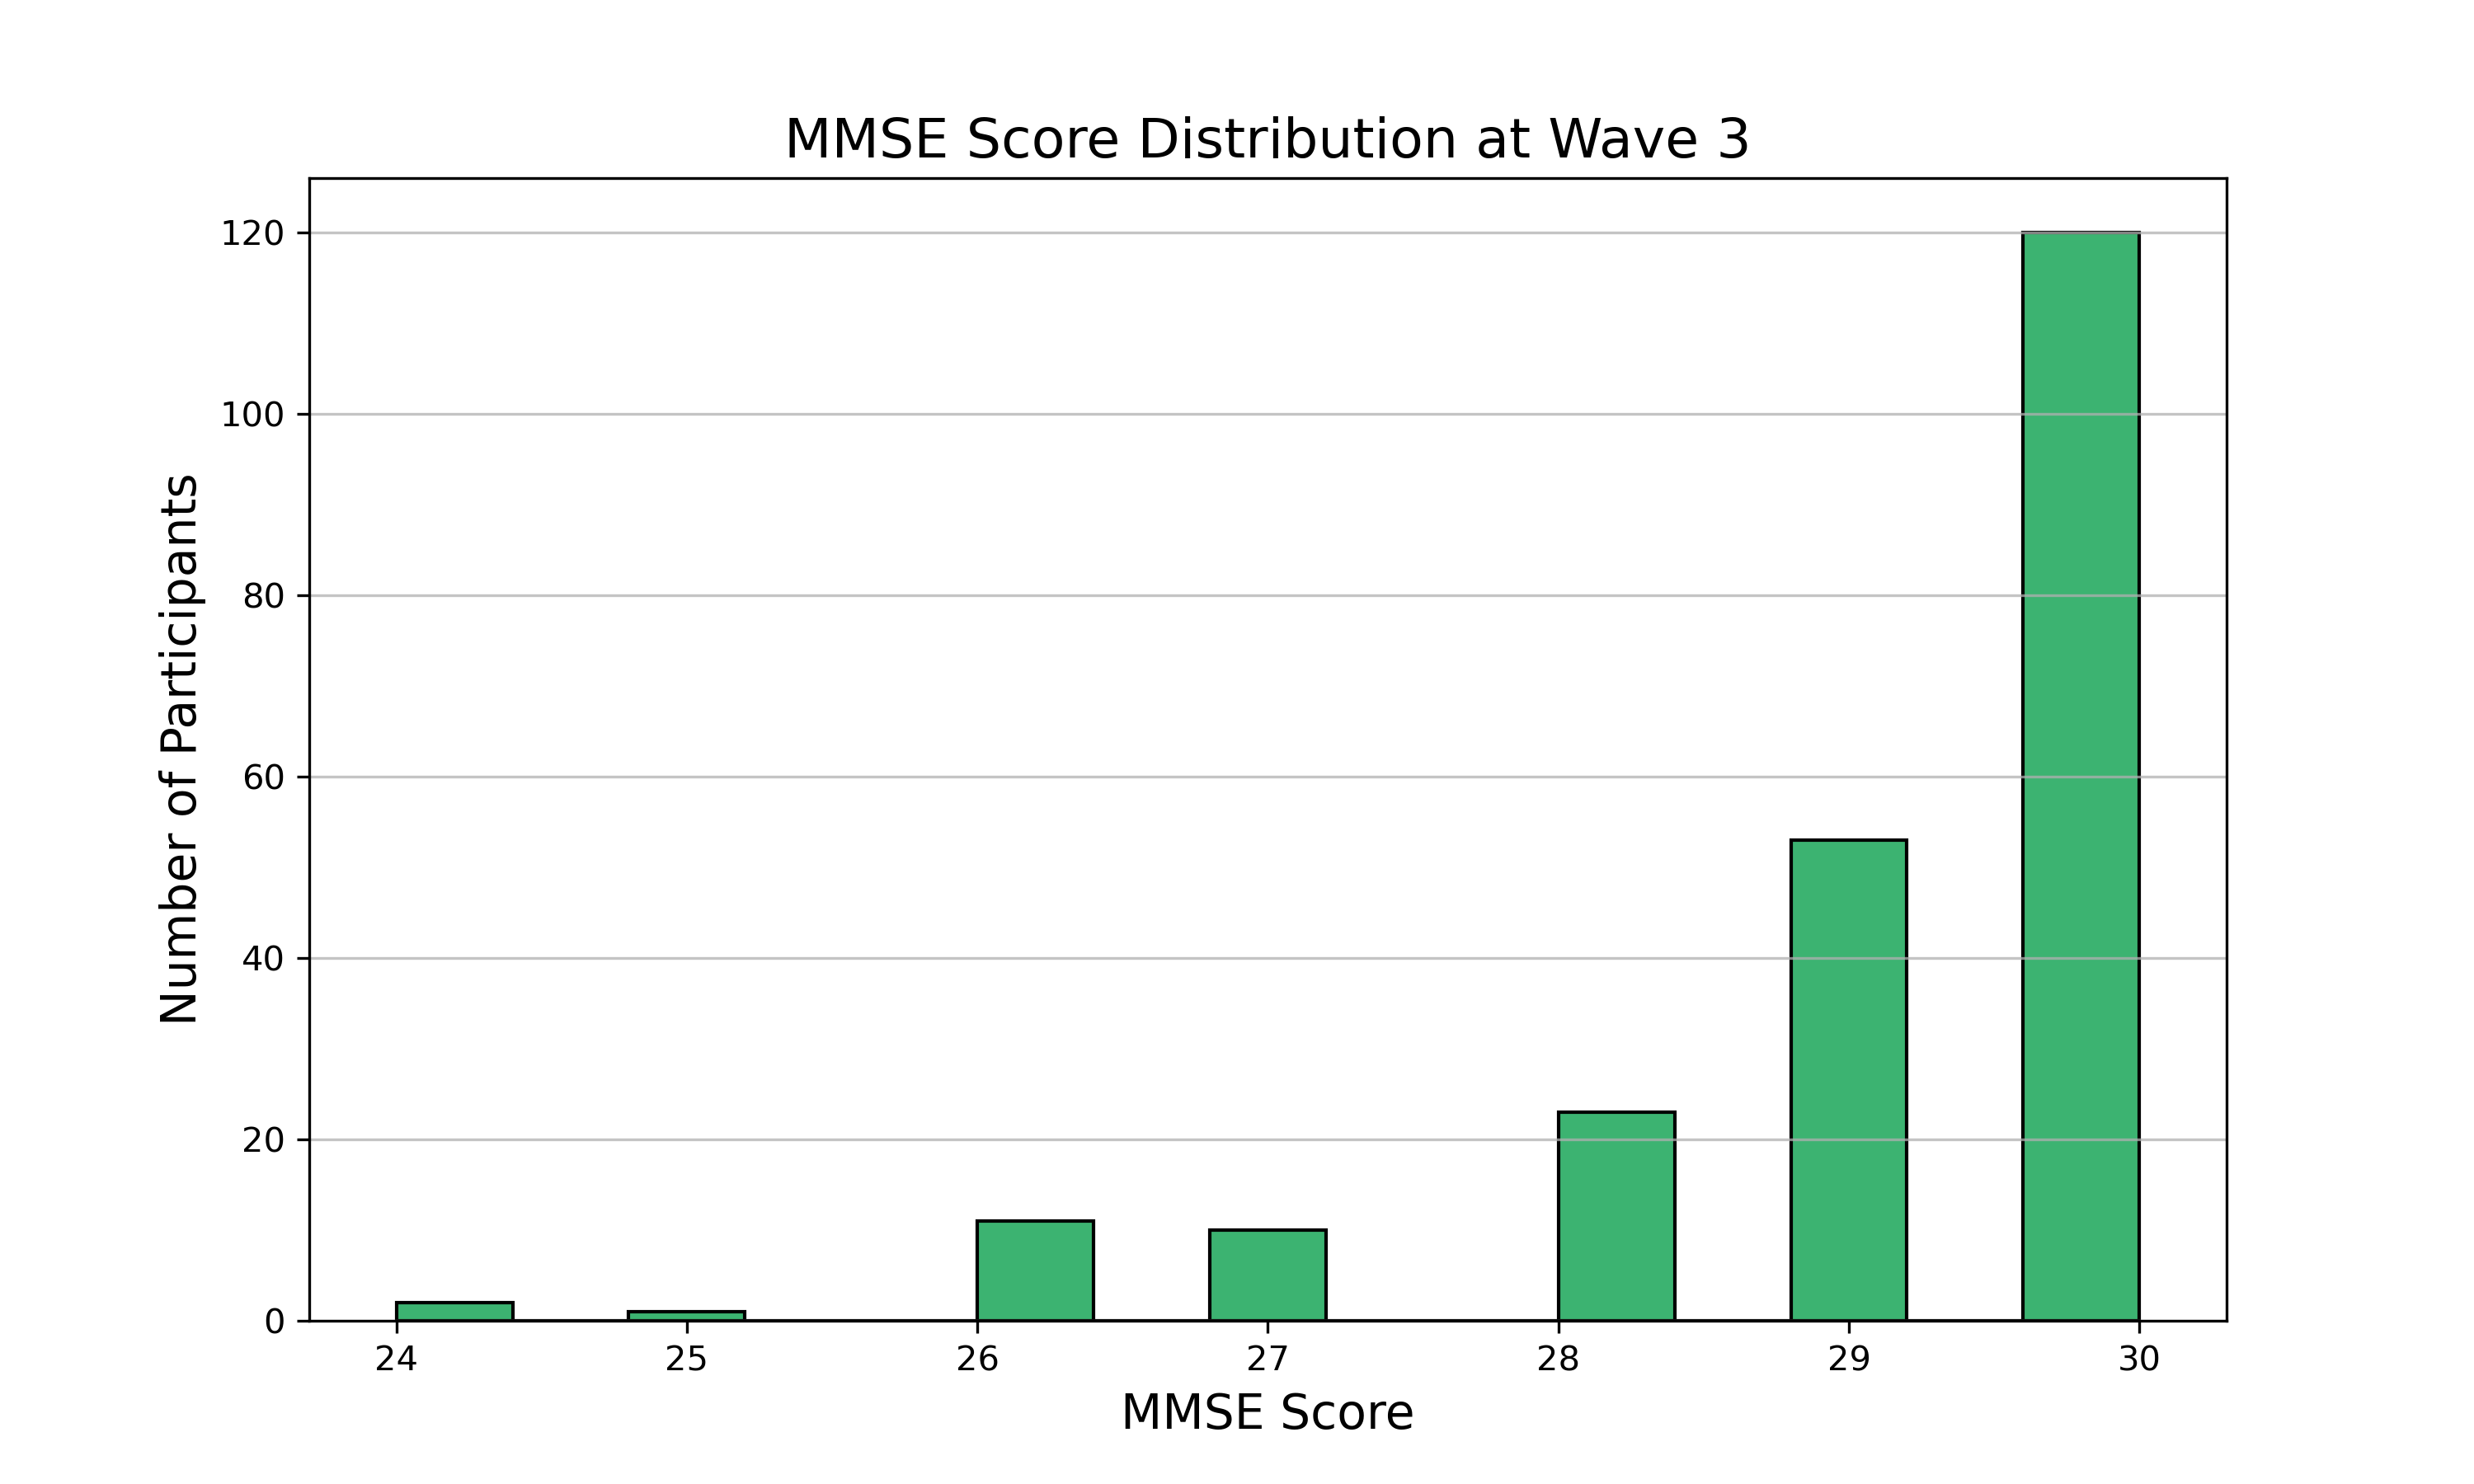
\includegraphics[width=0.8\linewidth]{mmse_w3_distribution.png}
    \caption{Histogram of MMSE scores at Wave 3}
  \end{figure}
\end{frame}

% Subsection: MRI Data
\subsection{MRI Data}

% Slide: MRI Protocol Summary
\begin{frame}{MRI Protocol in DLBS}
  \begin{itemize}
    \item \textbf{Structural MRI:} MPRAGE, FLAIR.
    \item \textbf{Functional MRI Tasks:}
      \begin{itemize}
        \item Ventral Visual Task
        \item Words Task
        \item Scenes Task
      \end{itemize}
    \item \textbf{Resting-State Imaging}
    \item \textbf{Diffusion Tensor Imaging (DTI)}
    \item \textbf{Arterial Spin Labeling (ASL)}
  \end{itemize}
\end{frame}

% Slide: Participants per Wave
\begin{frame}{Participants with MRI Data at Each Wave}
  \begin{figure}
    \centering
    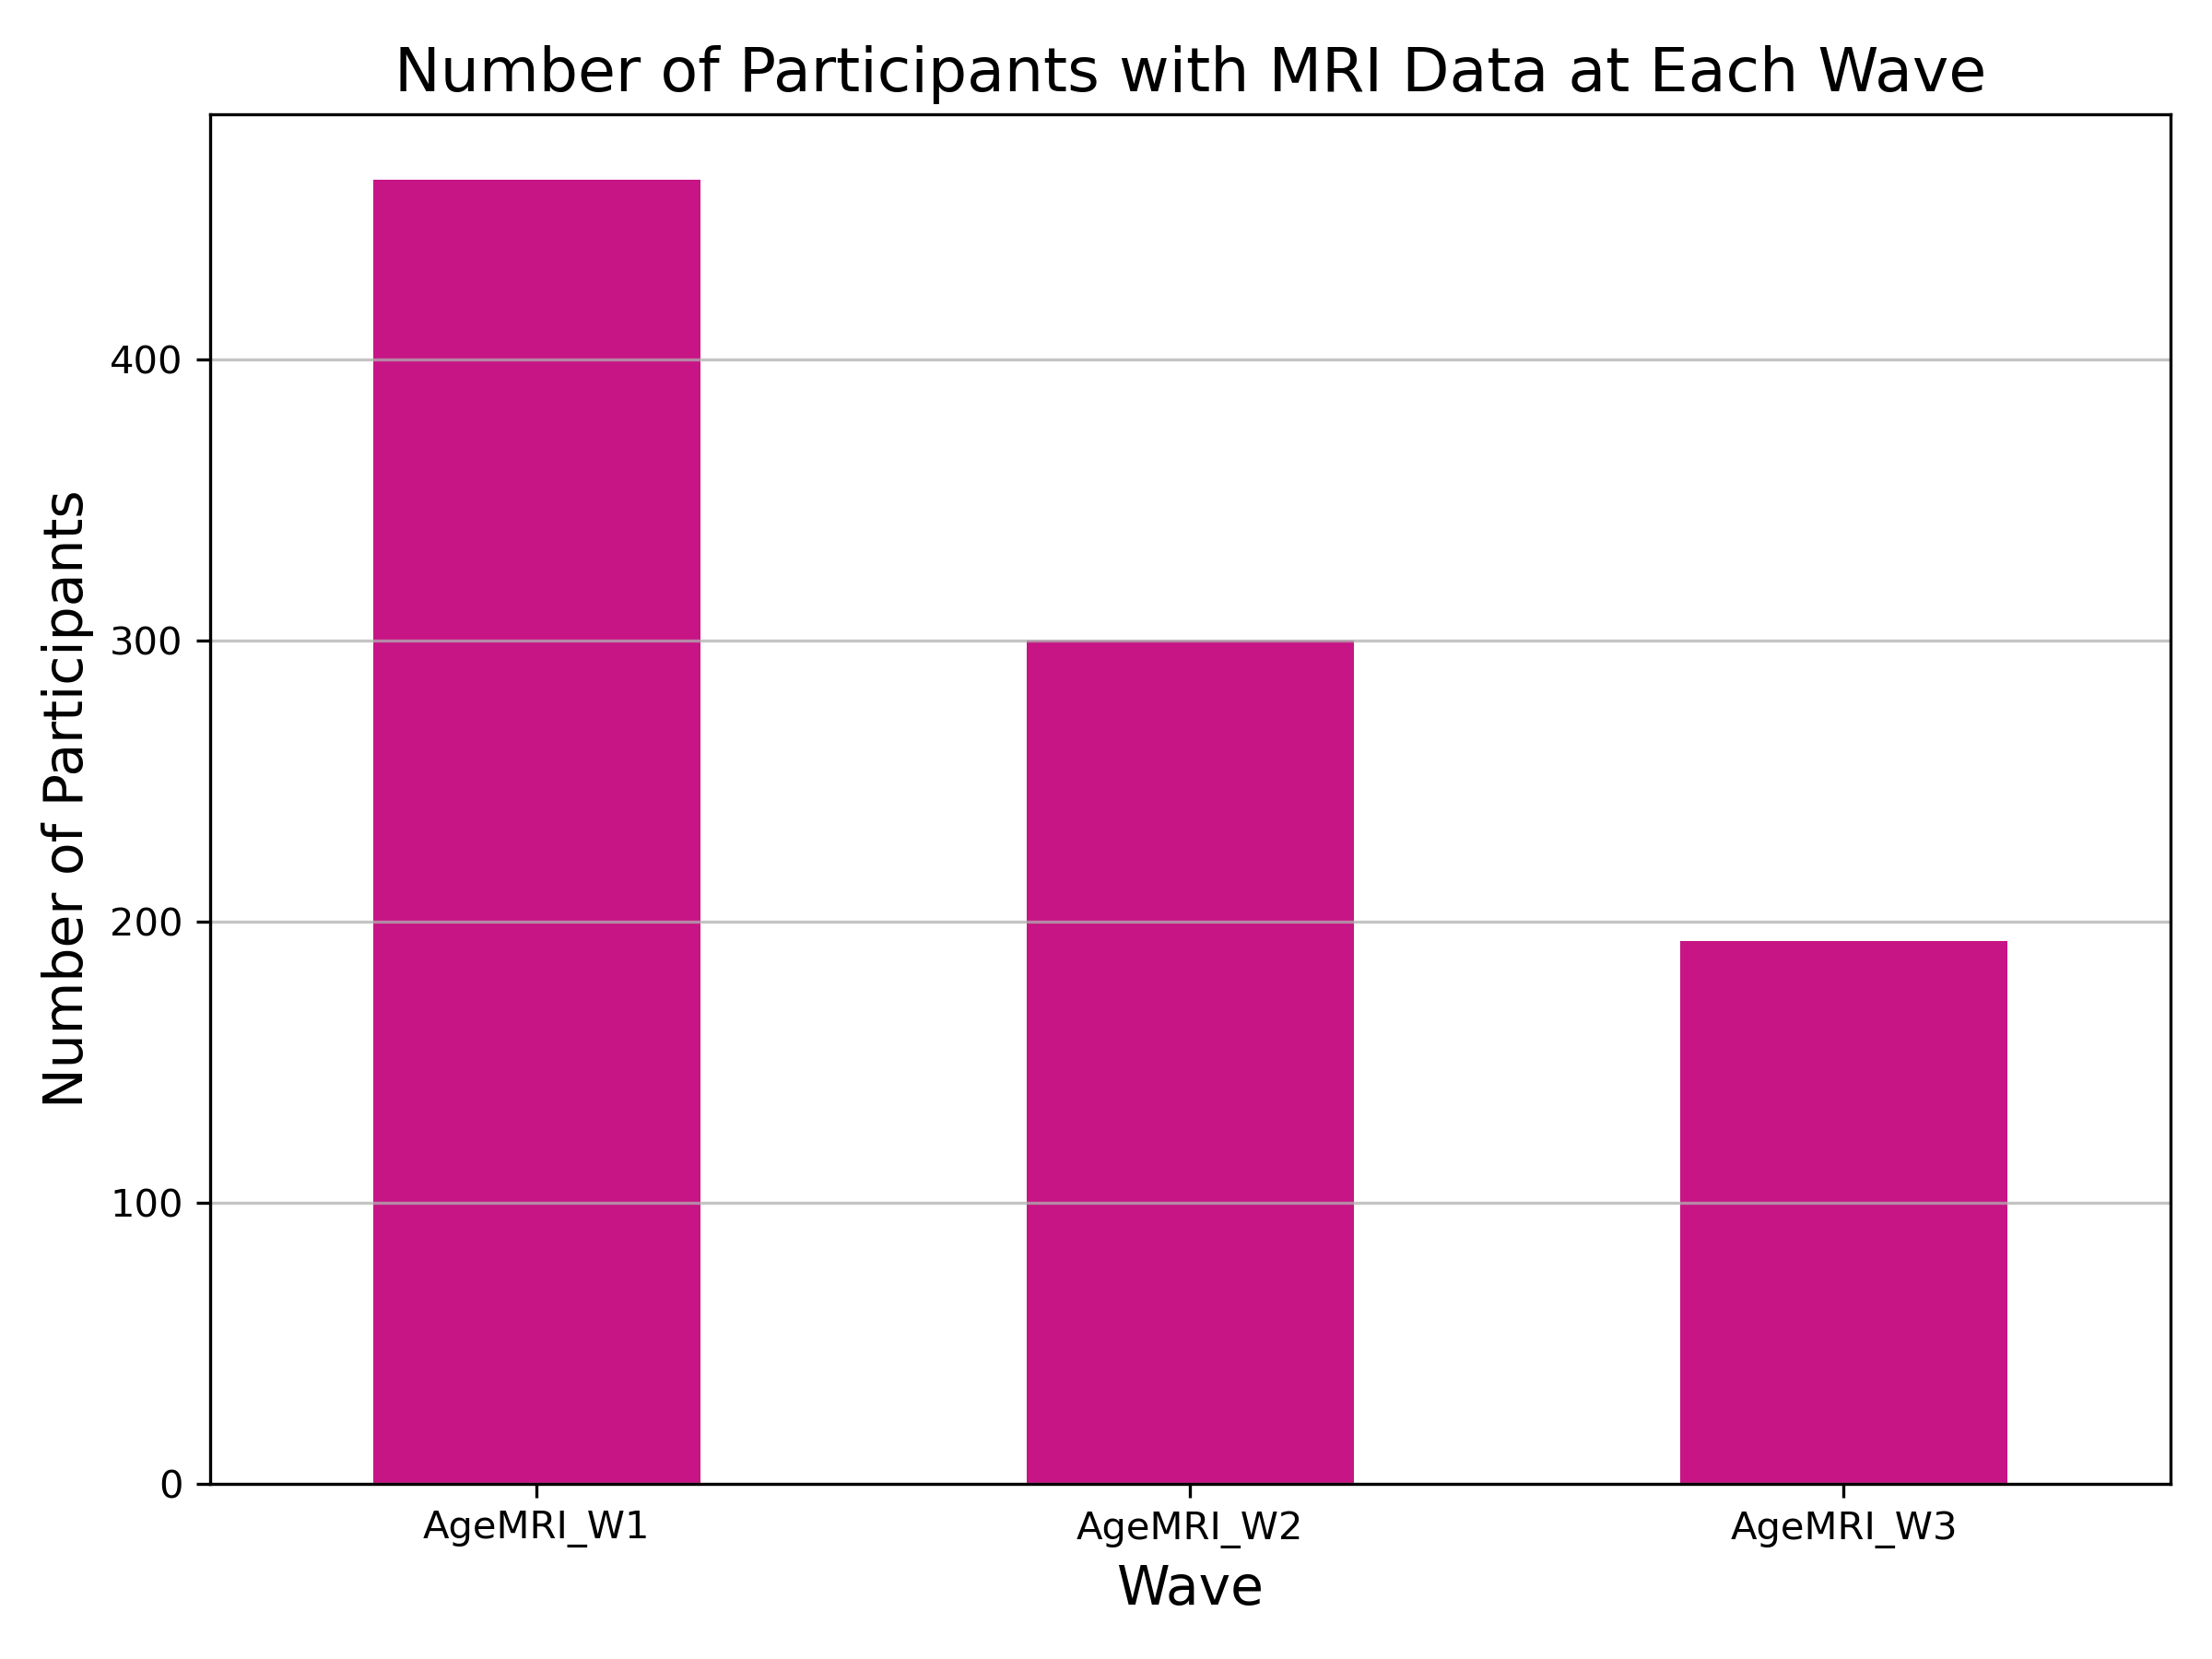
\includegraphics[width=0.6\linewidth]{participants_per_wave.png}
    \caption{Number of participants with MRI data at each wave}
  \end{figure}
\end{frame}

% Slide: Time Interval Between Wave 1 and Wave 2
\begin{frame}{Time Interval Between Wave 1 and Wave 2}
  \begin{figure}
    \centering
    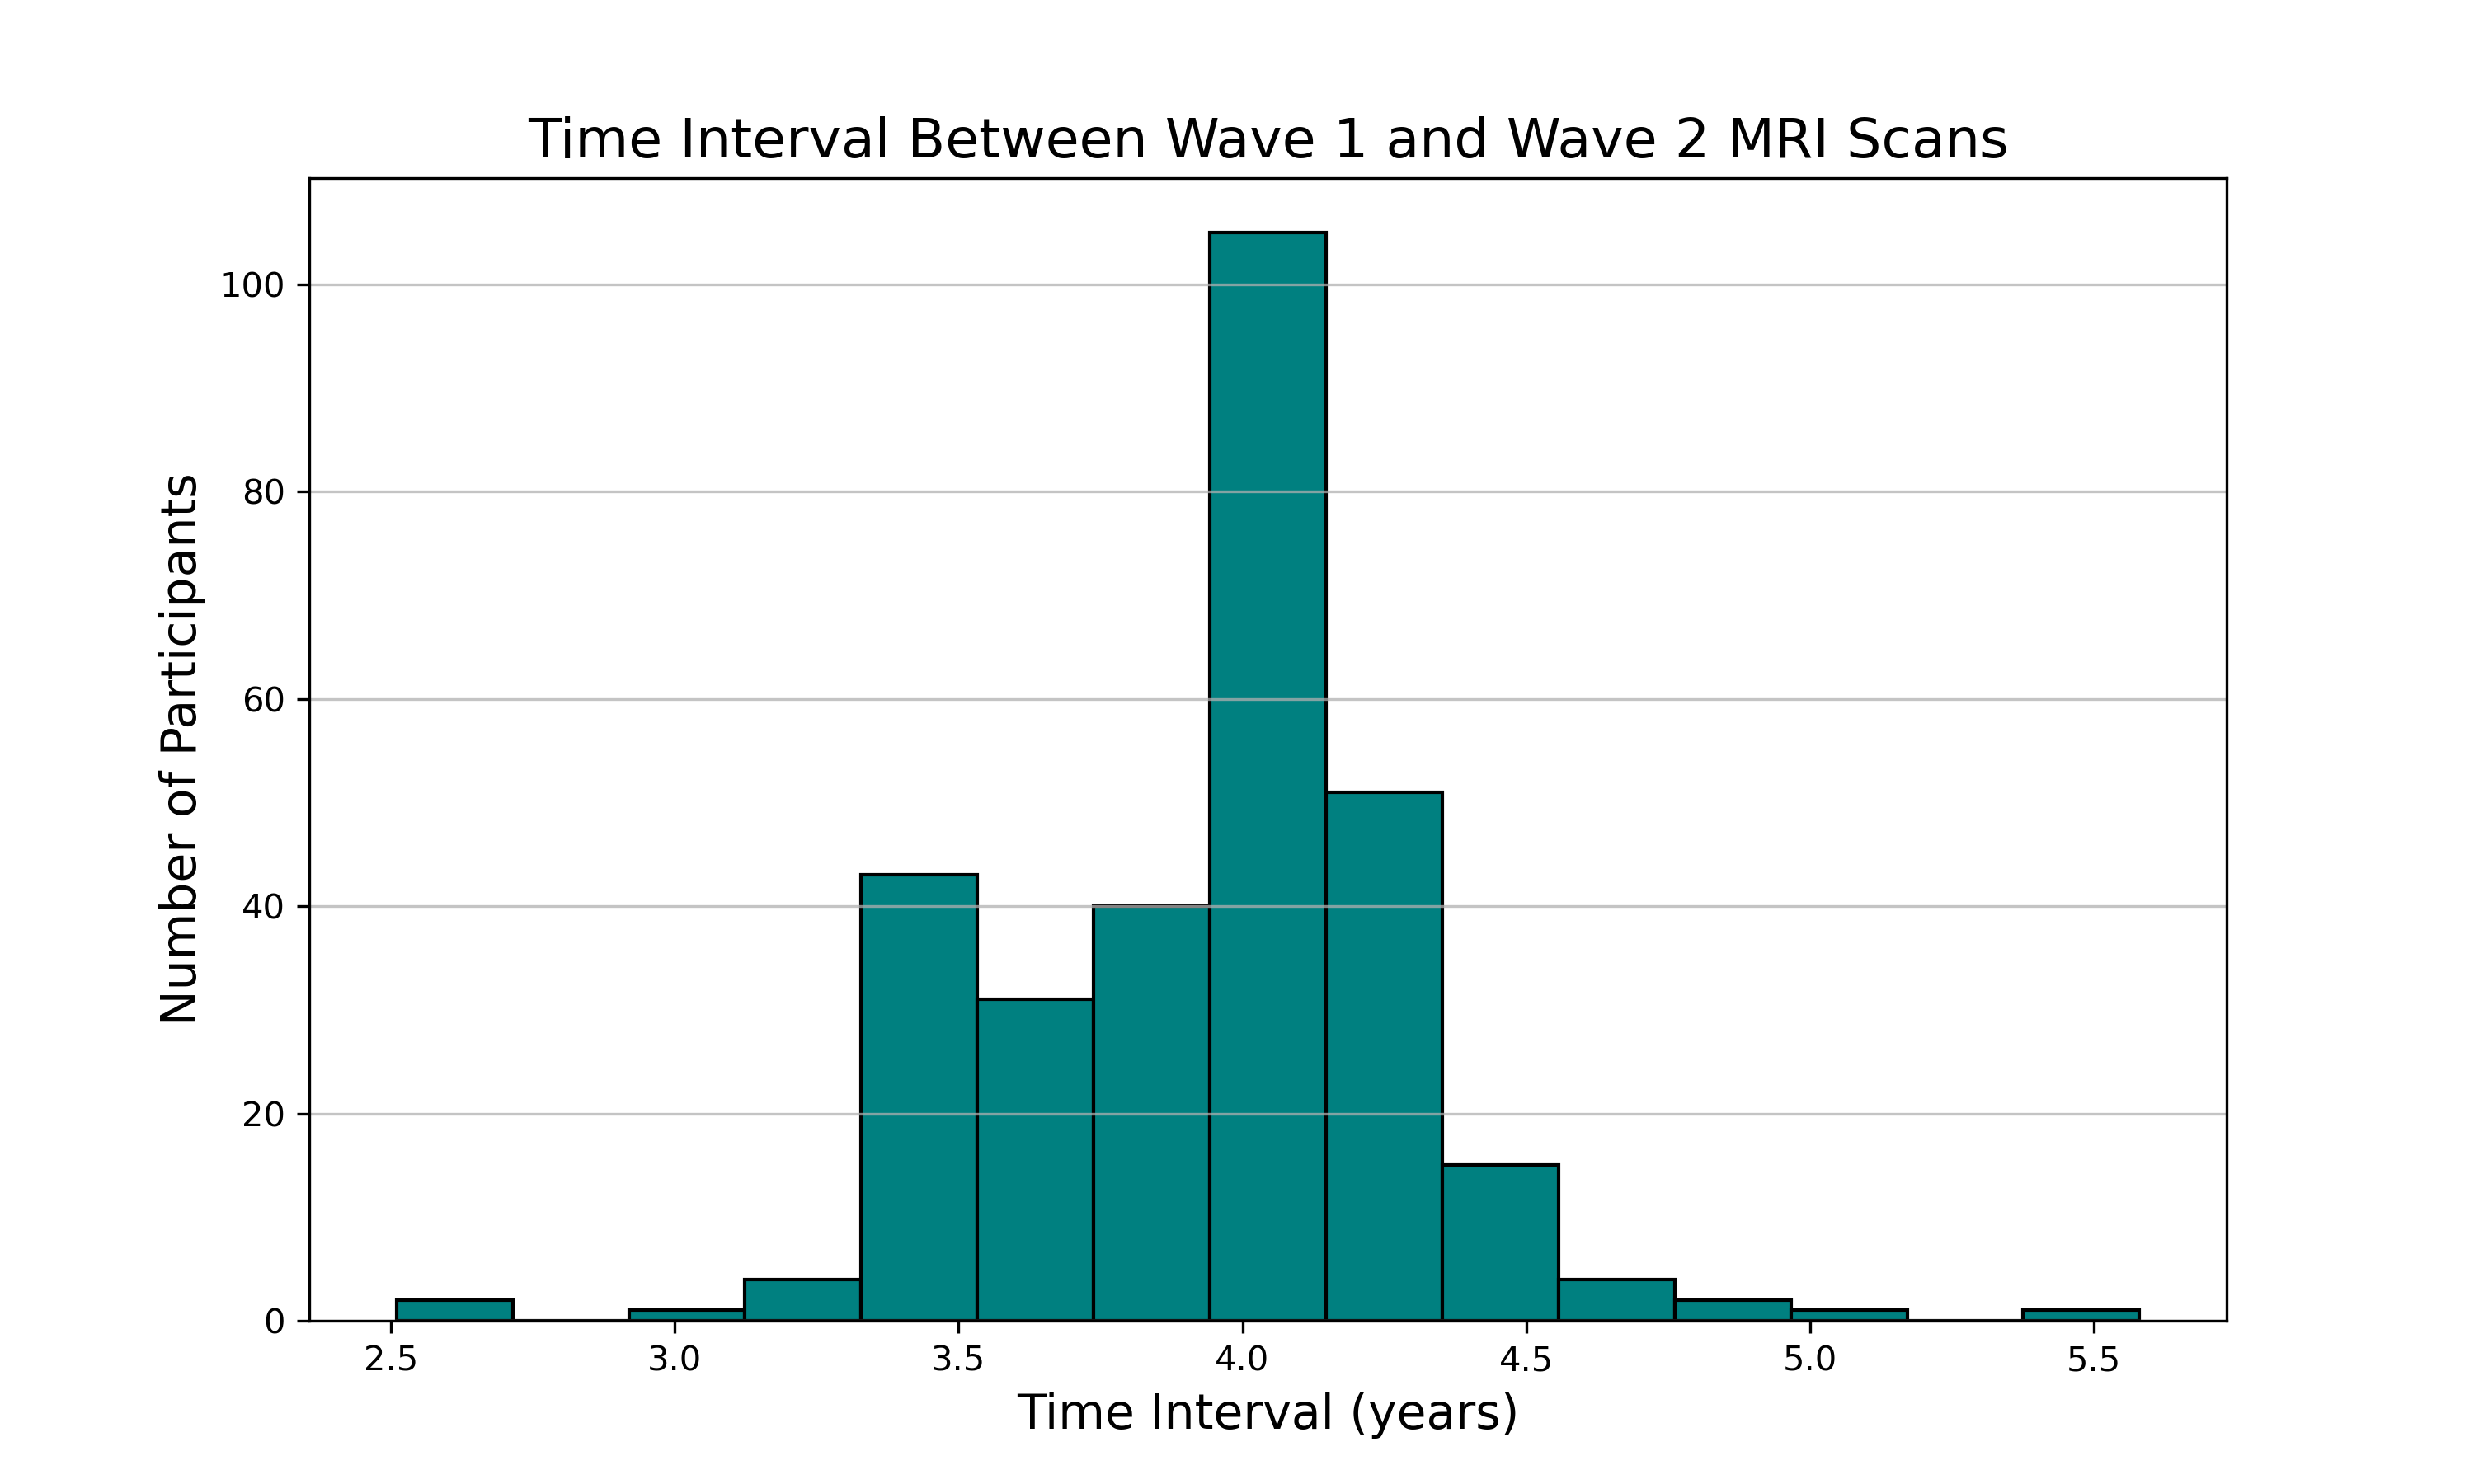
\includegraphics[width=0.8\linewidth]{mri_time_interval_w1_w2.png}
    \caption{Time interval between Wave 1 and Wave 2 MRI scans}
  \end{figure}
\end{frame}

% Slide: Time Interval Between Wave 2 and Wave 3
\begin{frame}{Time Interval Between Wave 2 and Wave 3}
  \begin{figure}
    \centering
    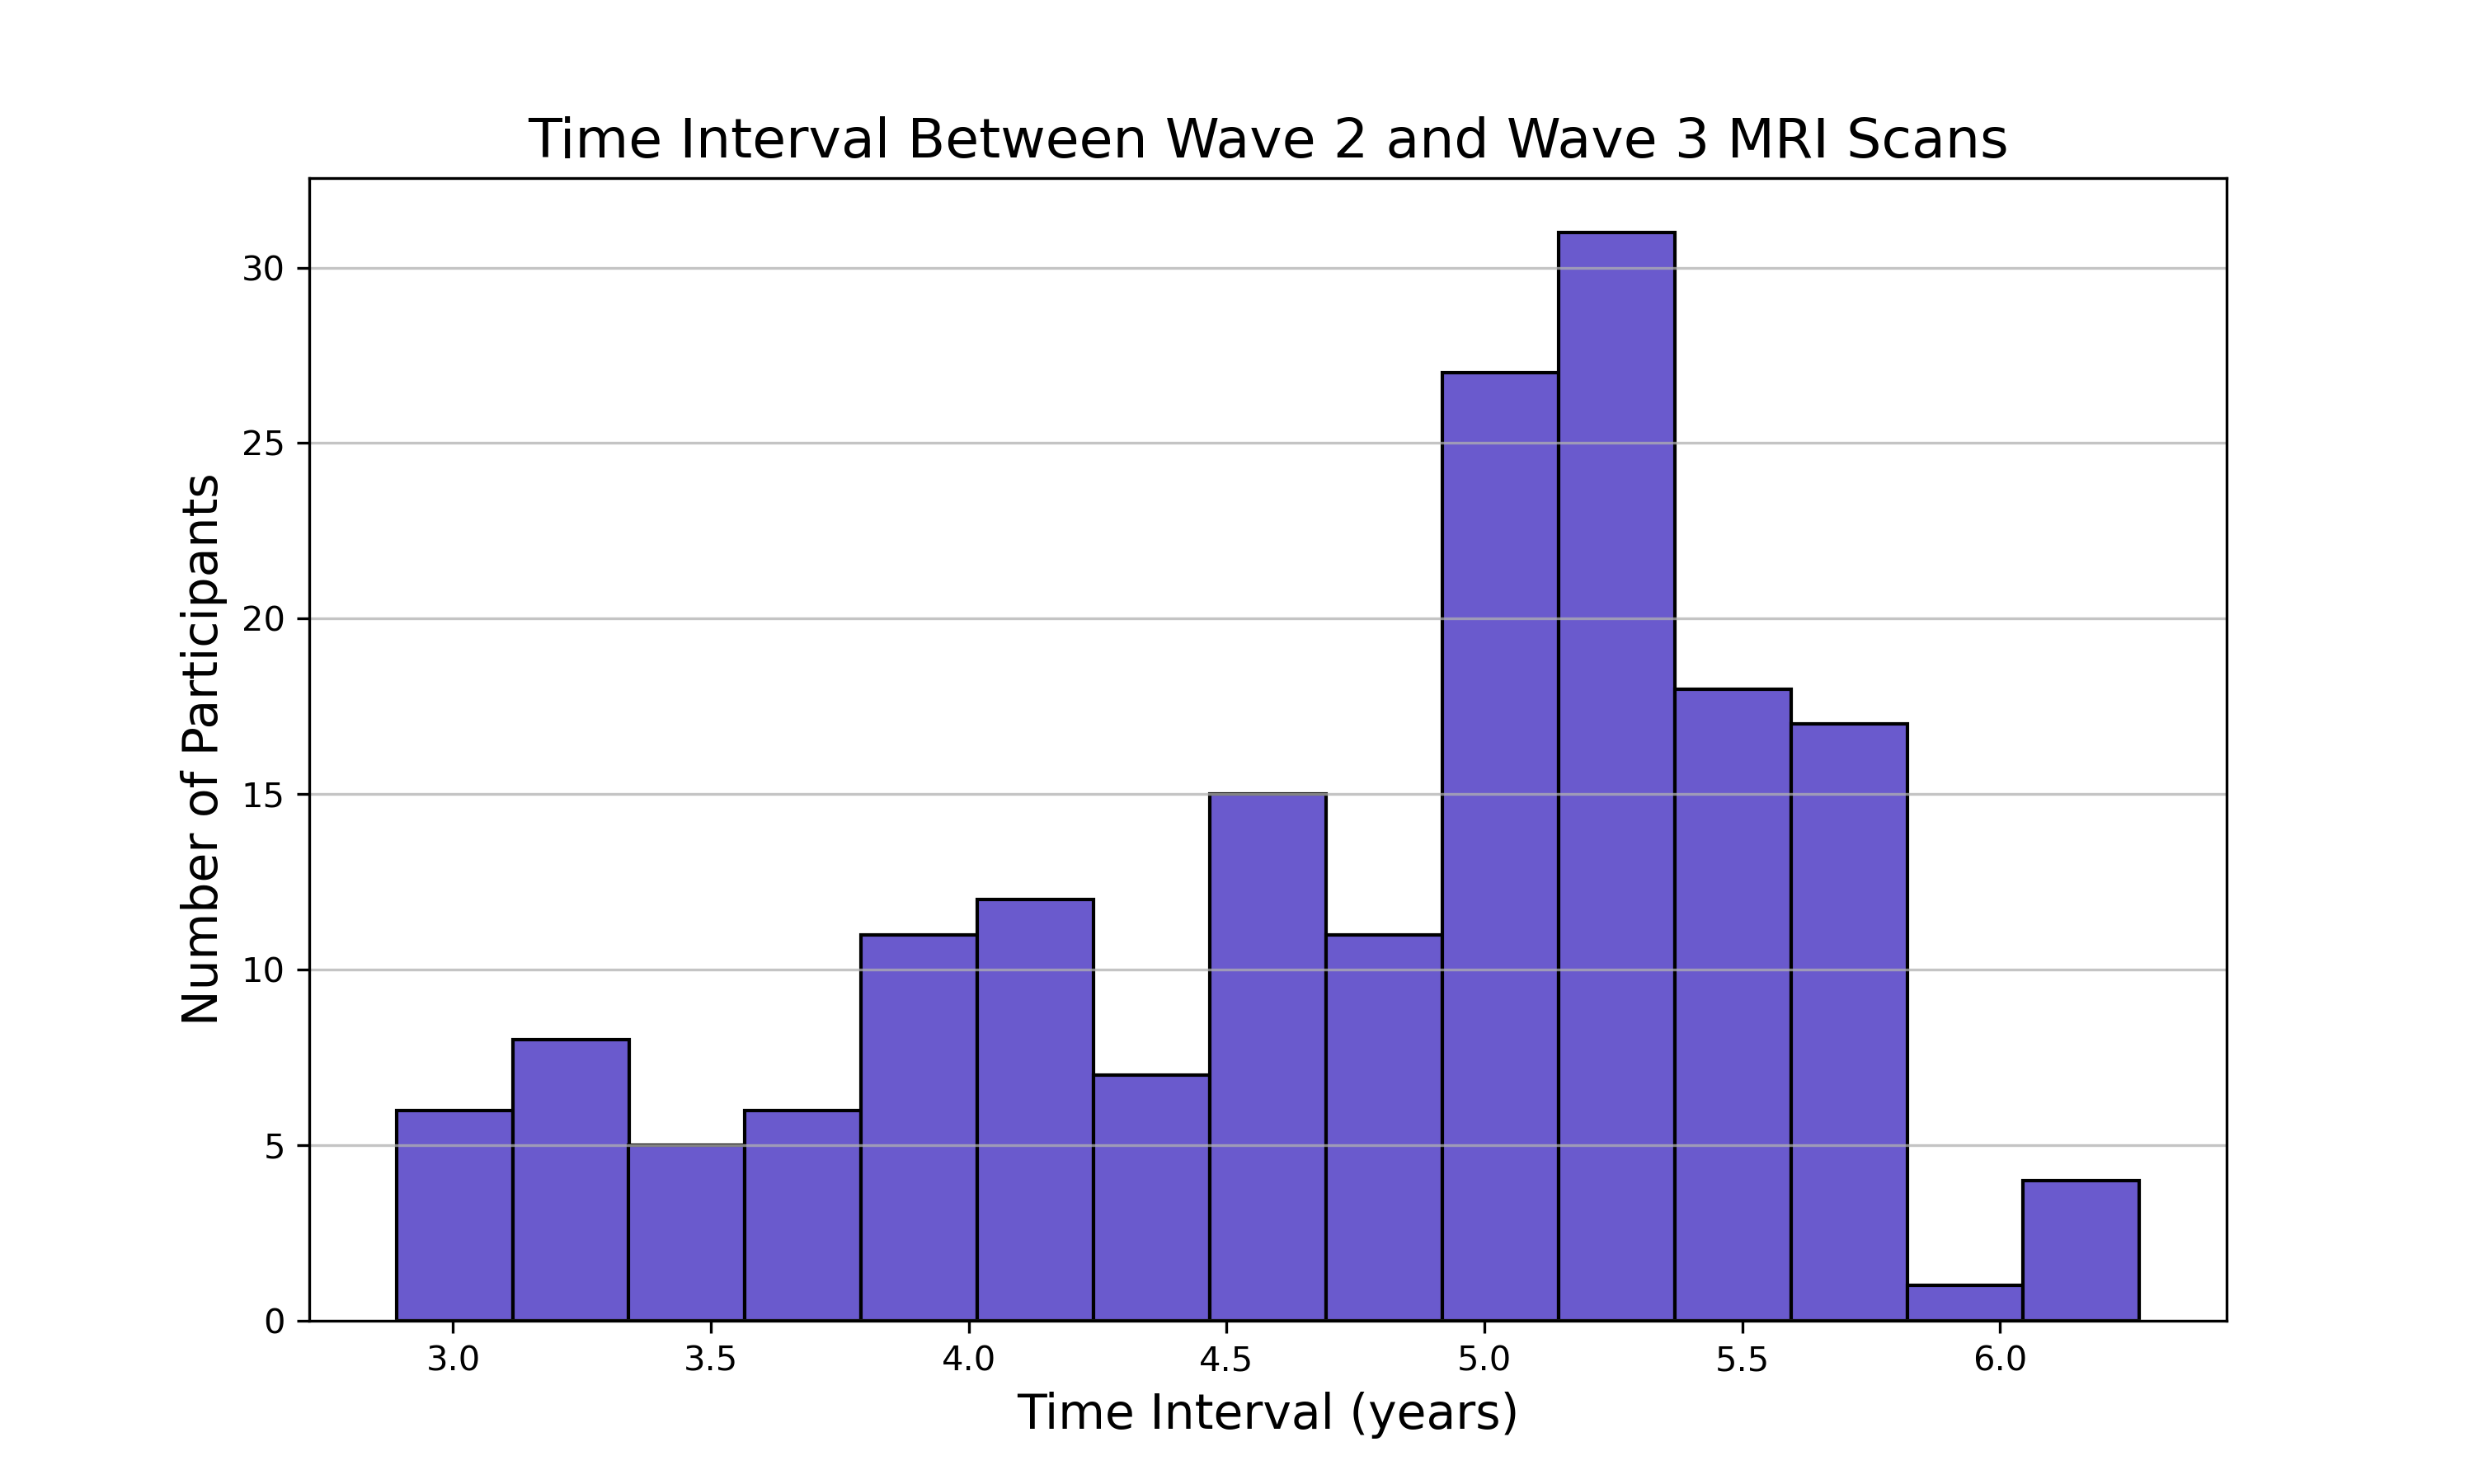
\includegraphics[width=0.8\linewidth]{mri_time_interval_w2_w3.png}
    \caption{Time interval between Wave 2 and Wave 3 MRI scans}
  \end{figure}
\end{frame}

% Slide: Correlation Matrix
\begin{frame}{Correlation Matrix of Participants Data}
  \begin{figure}
    \centering
    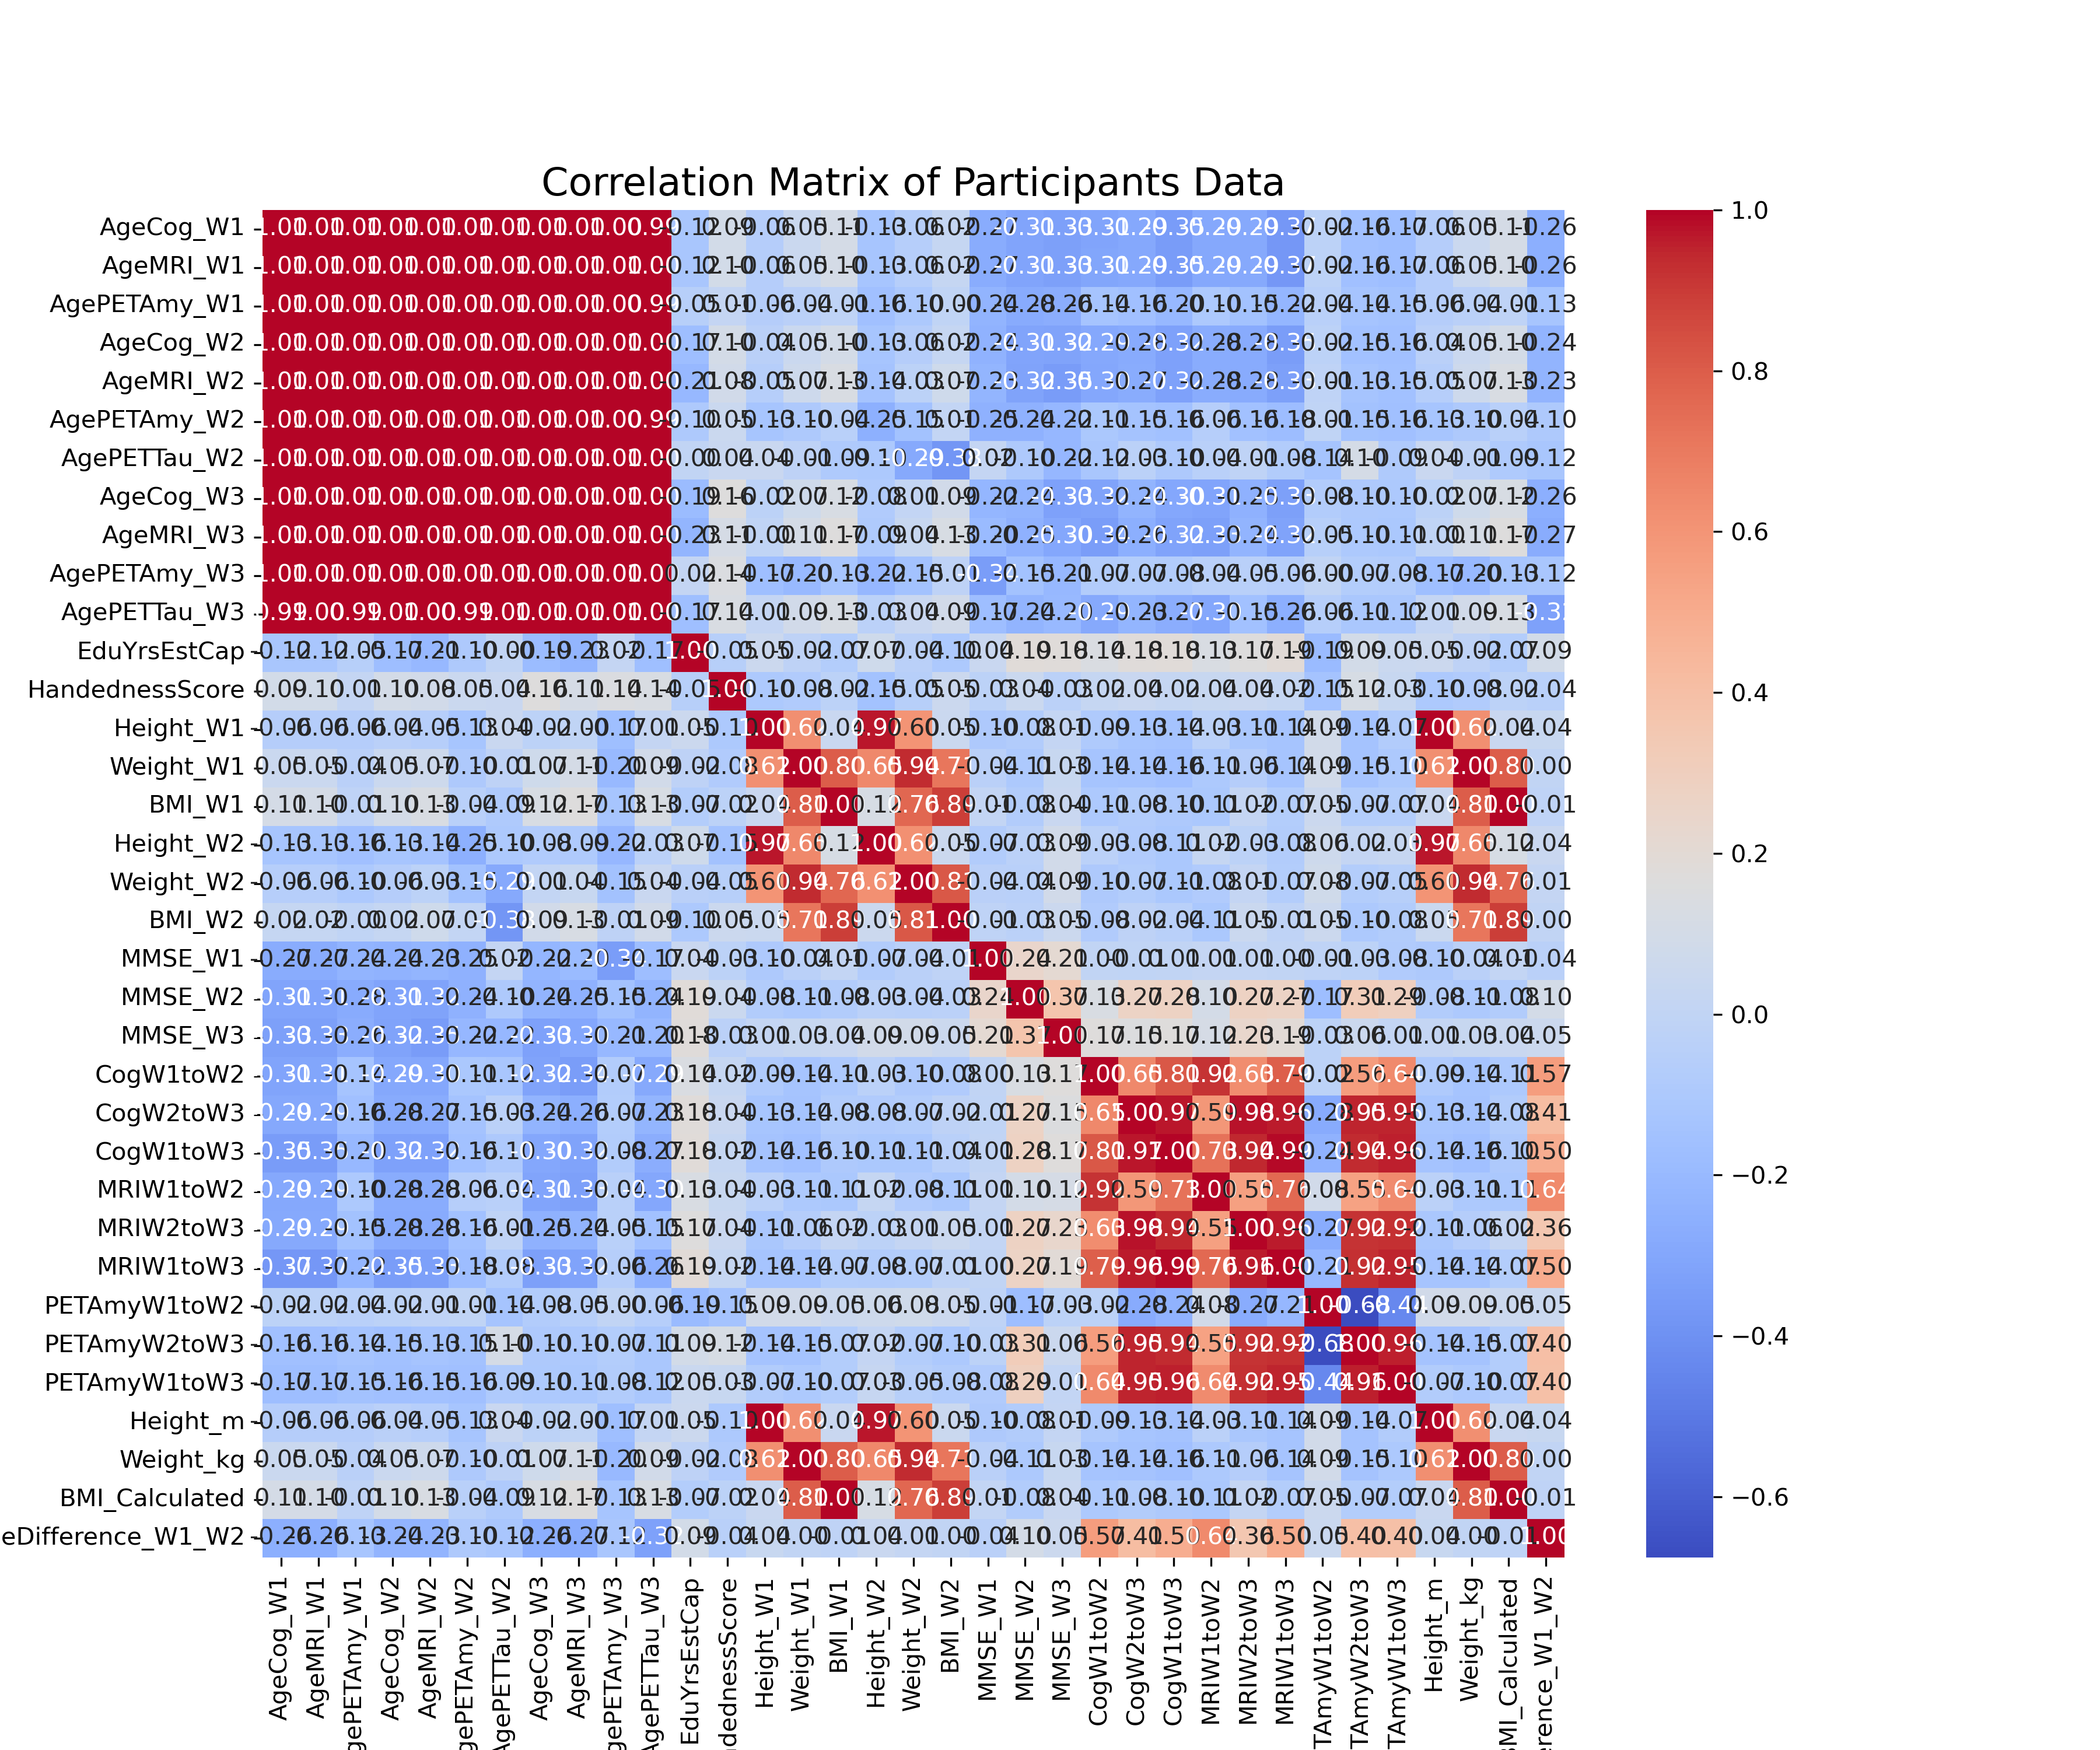
\includegraphics[height=0.8\textheight]{correlation_matrix.png}
    \caption{Heatmap of correlations among numerical variables}
  \end{figure}
\end{frame}

% Section: References
\section{References}
\begin{frame}[allowframebreaks]{References}
  \bibliographystyle{plain}
  \bibliography{references}
\end{frame}

\end{document}

